\documentclass[11pt,a4paper]{article}
\usepackage[utf8]{inputenc}
\usepackage{a4wide}
\usepackage{amsmath}
\usepackage{amsfonts}
\usepackage{amssymb}
\usepackage{graphicx}
\usepackage{float}
\usepackage{url}
\usepackage{amsmath}
%\usepackage[T1]{fontenc}
\usepackage{amsthm}
\usepackage{amssymb}
\usepackage[french,english]{babel}
\usepackage[babel=true,kerning=true]{microtype}
\usepackage[french]{cleveref}
\usepackage{svg}
\usepackage{caption}

\usepackage[left=3cm,right=3cm,top=3cm,bottom=3cm]{geometry}

\newtheorem{thm}{Theorem}
\newtheorem{prop}{Propriété}

\theoremstyle{definition}
\newtheorem{defn}{Définition}

\theoremstyle{remark}
\newtheorem{rmq}{Remarque}

\theoremstyle{remark}
\newtheorem{ex}{Exemple}

\def \stg {stream graph}
\def \Stgs {Stream graphs}
\def \Stg {Stream graph}
\def \stgm {stream graph multicouches}
\def \Stgm {Stream graph multicouches}
\def \stgs {stream graphs}
\def \stgms {stream graphs multicouches}
\def \Stgms {Stream graphs multicouches}


%tikz 
\usepackage{tikz}
\usepackage{pgfplots}
\usepackage{amsmath}
\usetikzlibrary{decorations.pathmorphing, positioning}
\definecolor{echoreg}{HTML}{2cb1e1}
\definecolor{echodrk}{HTML}{0099cc}
\tikzstyle{mybox} = [text=black, very thick,
    rectangle, rounded corners, inner sep=10pt, inner ysep=20pt]
\tikzstyle{fancytitle} =[text=black]
\newcommand{\yslant}{0.5}
\newcommand{\xslant}{-0.6}

%%%%%%%%%%%%%%%%%%%%%%%%%%%%%%%% TIKZ STYLES
\tikzstyle{every node}=[font=\scriptsize]

\tikzset{RootStyle/.style = {
						shape          = circle,
			      draw           = red!50!black!50,
			      thick,
			      top color      = white,
			      bottom color   = red!50!black!20,
			      text           = black,
			      inner sep      = .2pt,
			      outer sep      = 0pt,
			      minimum size   = 2.5 mm}
						}

\tikzset{VertexStyle/.style = {
						shape          = circle,
			      draw           = black!50,
			      top color      = white,
			      bottom color   = black!20,
			      text           = black,
			      inner sep      = .2pt,
			      outer sep      = 0pt,
			      minimum size   = 1.75 mm}
						}

\tikzset{EdgeStyle/.style   = {thick,<->}}

\tikzset{LabelStyle/.style =   {
				  text           = black,
				  inner sep      = .2pt,
				  outer sep      = 1pt,
				  font           =\scriptsize,
				  minimum size   = 2.15 mm}
					}

\pgfplotsset{compat=1.15}

\newcommand\overmat[3]{%
  \makebox[0pt][l]{$\smash{\color{#3}\overbrace{\phantom{%
    \begin{matrix}#2\end{matrix}}}^{\text{#1}}}$}#2}
\newcommand\undermat[3]{%
  \makebox[0pt][l]{$\smash{\color{#3}\underbrace{\phantom{%
    \begin{matrix}#2\end{matrix}}}_{\text{#1}}}$}#2}
\newcommand\partialphantom{\vphantom{\frac{\partial e_{P,M}}{\partial w_{1,1}}}}

\author{Pimprenelle Parmentier}



\title{Stream graphes multicouches}
\begin{document}
\selectlanguage{french}
\begin{titlepage}


\noindent
\textsc{Ecole polytechnique}\\
PROMOTION X2016 \\
MASTER: Mathématiques appliquées\\
PARMENTIER Pimprenelle

\vspace{3cm}
\begin{center}
\textsc{\Large Rapport de stage}
\vspace{1cm}
\hrule % Horizontal line
\vspace{0.4cm}
{\huge \bfseries \Stgms \par}\vspace{0.4cm} % Thesis title
\hrule 
\vspace{1cm}
\textsc{\Large Rapport non confidentiel}
\vspace{4cm} % Horizontal line
 
\end{center}

\noindent
\textit{Option:} Mathématiques appliquées\\
\textit{Champ:} Recherche opérationnelle, théorie des graphes\\
\textit{Enseignant référent:} Xavier \textsc{Allamigeon}\\
\textit{Tuteur de stage dans l'organisme:} Tiphaine \textsc{Viard}\\
\textit {Co-tuteurs de stage hors organisme:} Benjamin \textsc{Renoust} (Université d'Osaka)\\
\hspace*{3.1cm} Jean-François \textsc{Baffier} (Japan Society for the Promotion of Science)\\
\textit{Dates du stage:} 8 avril 2019 - 23 aout 2019\\
\textit{Adresse de l'organisme:}\\
RIKEN AIP\\
Nihonbashi 1-chome \\
Mitsui Building, 15th floor,\\
1-4-1 Nihonbashi,\\
Chuo-ku, Tokyo\\
103-0027, Japan\\
\end{titlepage}

\section*{Déclaration d’intégrité relative au plagiat}

Je soussignée \textsc{Parmentier} Pimprenelle certifie sur l’honneur:

\begin{enumerate}
    \item Que les résultats décrits dans ce rapport sont l’aboutissement de mon travail.
    \item Que je suis l’auteur de ce rapport.
    \item Que je n’ai pas utilisé des sources ou résultats tiers sans clairement les citer et les
référencer selon les règles bibliographiques préconisées.
\end{enumerate}

Mention à recopier

\textit{Je déclare que ce travail ne peut être suspecté de plagiat.}

\vspace{2cm}
Date: .................................. \hspace{2cm} Signature:

\newpage

\begin{abstract}

Ce rapport de stage traite d'un nouvel objet permettant d'étudier des graphes complexes dépendants du temps : les \textbf{\stgms{}}. 

Dans un premier lieu, nous faisons un état de l'art sur les formalismes existants pour traiter de graphes complexes et de graphes temporels. Nous présentons ainsi les graphes multicouches et les \stgs{} qui nous servent à construire les \stgms{}. 

Dans un second temps, nous donnons une définition formelle des \stgms{}, et nous montrons en quoi ce nouvel objet est une généralisation des objets existants. Puis nous définissons des mesures permettant d'étudier les \stgms{}, qui prennent en compte l'aspect à la fois multicouches et temporel.

Nous présentons ensuite la bibliothèque Python con\c{c}ue pour traiter ce type d'objet, ainsi qu'un exemple d'utilisation avec un jeu de données temporel multicouches.

Enfin, nous donnons un ensemble de pistes que nous pourrons explorer pour la suite du stage.

\end{abstract}



\selectlanguage{english}

\begin{abstract}

This internship report is about a new object that deals with time-dependant complex graphs: the multilayer stream graphs. 

First of all, we present the state-of-the-art on the existing formalisms that handle complex graphs and temporal graphs. We present multilayer graphs and stream graphs, on the basis of which we build the multilayer stream graphs.

Then, we give a formal definition of multilayer stream graphs, and we demonstrate that it as a generalisation of existing objects. We define measures to study the multilayer stream graphs, which takes into account both multilayer and temporal aspects.

We also introduce a Python library designed to handle this type of object, as well as an example of use with a multilayer temporal dataset.

Finally, we give a set of tracks that we can explore for the rest of the internship.

\end{abstract}

\selectlanguage{french}
\newpage 

\tableofcontents
\newpage


\section*{Remerciements}

    En premier lieu, je souhaite remercier ma tutrice Tiphaine \textsc{Viard}, qui a rendu mon stage possible, ainsi que mes co-tuteurs Jean-François \textsc{Baffier} et Benjamin \textsc{Renoust} pour leur accompagnement pendant la durée du stage. Grâce à leurs conseils et leur suivi, j'ai pu apprendre beaucoup de choses dans le domaine des graphes mais également sur la recherche en général.
    
    Je remercie également les équipes administratives de RIKEN et de l'École Polytechnique pour leur support.

\newpage

\section*{Introduction}

    Un graphe représente un ensemble d'entités (des n\oe{}uds), reliés par des liens. Ces données sont omniprésentes: des villes sont liées par des routes, des personnes par des relations d'amitié, etc. La première formalisation du concept remonterait à Euler, en 1750, qui énonça le problème des ponts de Köningsberg~\cite{wikigraphes,divin}. Cet objet a permis de nombreuses avancées dans plusieurs domaines: en algorithmique, en probabilités, en combinatoire, en optimisation ou plus récemment, pour l'analyse de données massives du monde réel (graphes de terrain).
    
    La puissance de la théorie des graphes vient du fait qu'elle permet d'exprimer des problèmes réels variés dans un même formalisme très synthétique, auquel on applique des algorithmes spécifiques permettant d'accéder à de nombreux résultats. Malgré la simplicité apparente du modèle, ces résultats sont subtils, et très utilisés à l'heure actuelle (PageRanking~\cite{pr}, plus court chemin~\cite{dijkstra}, \textit{etc}).
    
    Ce formalisme peut être étendu pour capturer de la diversité dans les données : les liens peuvent être dirigés, pondérés, étiquetés, \textit{etc}. Cependant, l'extension de ces notions sur ces graphes est loin d'être triviale, ce qui appelle à l'élaboration de nouveaux formalismes. Par ailleurs, de nombreuses données se présentent sous la forme d'interactions plutôt que de relations: cela peut être des ordinateurs qui échangent des paquets, ou encore des chercheurs collaborant sur un sujet. Ces interactions comportent par nature une dimension temporelle. Des données peuvent également présenter des structures particulières: par exemple, des villes sont liées par différentes moyens de transport, ou encore nous pouvons nous intéresser à des banques implantées dans différents pays procédant à des transactions. 
    
    Notre objectif ici est d'élaborer un formalisme généralisant l'existant afin de représenter des interactions dépendant du temps, tout en prenant en compte la structure des n\oe{}uds et des liens: nous appelons cet objet le \stgm{}\footnote{La traduction du terme anglais scientifique \og stream graph \fg{} n'étant pas définie lors de la rédaction de ce rapport, nous avons décidé de le conserver dns la langue anglaise pour éviter toute ambiguité.}.
    
    
    Dans une première partie, nous établissons l'état de l'art en rappelant les définitions pertinentes des graphes, des graphes multicouches et des \stgs{}, et nous explorons les limites associées à ces formalismes. Ensuite, nous présentons et nous formalisons les \stgms{}, ainsi que les définitions associées. Nous explorons en détail les relations entre notre formalisme et les théories existantes, notamment par le biais de projections qui nous définissons.
    
    L'applicabilité de notre formalisme à des données réelles est cruciale et c'est pour cela que nous présentons une implémentation au \cref{application}, ainsi que les résultats obtenus sur un premier jeu de données.
    
    Enfin, nous évoquerons des perspectives ouvertes par ce travail.
	
\section{Etat de l'art : deux formalismes sur les graphes}
\indent

Dans cette partie, nous présentons les objets qui ont servi à construire les \stgms{}: tout d'abord les \textbf{graphes}, puis les \textbf{graphes multicouches} qui servent à traiter de graphes à structure complexe, et les \textbf{\stg{}s} qui permettent de modéliser des séquences d'interactions.

\subsection{Graphes}

Un \textbf{graphe simple} $G$ est un ensemble de n\oe{}uds $V$ ainsi qu'un ensemble d'arêtes $E \subseteq V \otimes V$, chaque élément de $E$ étant une paire non ordonnée de deux éléments de $V$. Les arêtes représentent une interaction entre deux n\oe{}uds. De façon générale, on désigne $V\otimes V$ l'ensemble des paires $\{u,v\}$ non ordonnées d'éléments de $V$ où $u \neq v$. 


Nous avons donné ici la version la plus basique des graphes, mais il existe de nombreuses variantes; on peut prendre une paire ordonnée (les paires ordonnées de $V$ sont écrites $(u,v) \in V\times V$) et on obtient un graphe dirigé, associer une fonction de poids à chaque lien (graphes pondérés), etc.


\begin{figure}[h]
			\begin{center}
					\begin{tikzpicture}[xscale=2,yscale=2,auto]
							\draw (2,0) node[VertexStyle]   (A) { A };
							\draw (0,0) node[VertexStyle] (B) { B };
							\draw (0,2) node[VertexStyle]   (C) { C };
							\draw (2,2) node[VertexStyle]   (D) { D };

							\draw[EdgeStyle]				(B) to node[LabelStyle]{}	(A);
							\draw[EdgeStyle,bend left=40,looseness=1.1]    	(C) to node[LabelStyle]{}   	(A);
							\draw[EdgeStyle] 	(C) to node[LabelStyle]{}     	(B);
							\draw[EdgeStyle]  	(C) to node[LabelStyle]{} 		(D);
							

					\end{tikzpicture}
			\end{center}
	\caption{Un exemple de graphe $G=(V,E)$ avec $V=\{A,B,C,D\}$ et $E=\{AB,AC,BC,DC\} $. Il représente des relations entre divers individus de la même espèce. Un lien existe entre deux animaux s'ils ont été en contact. }
	\label{fig:tikzminimal}
\end{figure}


%Comme dit en introduction, la théorie des graphes permet de modéliser et de résoudre de nombreux problèmes de la vie réelle, en synthétisant des informations. Ces problèmes sont étudiés depuis plus de 200 ans et nous avons à présent de nombreux outils pour les étudier, même si le domaine est encore en évolution.

La théorie des graphes permet d'analyser des jeux de données à un niveau assez fin.

Par exemple, les mesures de \textbf{centralité} permettent de détecter quels sont les n\oe{}uds les plus \og influents \fg{}. Il en existe plusieurs types, de plus en plus \og fins \fg{}. Le {\em degré} qui est le nombre d'arêtes incidentes à n\oe{}ud, est la première. Ensuite, on trouve la centralité d'intermédiarité ({\em betweeness centrality})~\cite{centralities}, dans laquelle on calcule combien de fois le n\oe{}ud est présent dans les plus courts chemins entre toutes les paires du graphes. Enfin, dans des graphes orientés, on simule des marches aléatoires entre les n\oe{}uds du graphe et mesurer vers quels n\oe{}uds elles convergent~\cite{pr}.
Un autre exemple est le \textbf{partitionnement spectral}~\cite{clustering}, permettant de diviser l'ensemble des n\oe{}uds en plusieurs sous-ensembles (clusters) distincts, de sorte à minimiser le nombre d'arêtes entre deux sous-ensemble différents (ce nombre est appelé \og coupe \fg{}).

\subsection{Les graphes multicouches}

Les graphes permettent de synthétiser et de représenter des relations entre individus. Un seul type de relations entre un seul type d'individus peut être représenté, soit en ignorant leurs différences, soit en ne représentant qu'une partie des relations et des n\oe{}uds. 

Les graphes multicouches permettent de pallier à cette perte d'informations.

\subsubsection{Définition générale}

 Les graphes multicouches~\cite{mlkiv} sont utilisés pour décrire des interactions entre des n\oe{}uds qui peuvent être de différentes natures et/ou qui peuvent avoir des interactions de natures différentes. 
 
 
 
  Un \textbf{graphe multicouches} est un quadruplet $M = (V_M, E_M, V, {\cal L})$.
  
 Sa {\em structure} est décrite par le k-uplet d'ensembles ${\cal L} = L_1, \dots , L_k$. Chaque $L_i$, appelé {\em aspect}, est un ensemble d'attributs, appelés {\em couches élémentaires}. Chaque {\em couche} correspond à un élément de $L=L_1\times L_2 \times \dots \times L_k$.\label{structure}
 
 $V$ est l'ensemble des {\em n\oe{}uds}, l'ensemble $V_M \subseteq V\times L$ les {\em n\oe{}uds-couches}. Enfin $E_M \subseteq V_M \otimes V_M $ est l'ensemble des {\em arêtes}, une arête pouvant relier deux n\oe{}uds-couches entre eux. 


 La \cref{exmulti} donne un exemple de graphe multicouches.

\begin{figure}[h]
	\centering
	
%0.58
\begin{tikzpicture}[scale=0.38,every node/.style={minimum size=1cm},on grid]

	\node [mybox, scale=1.0] at (10.5, 2) (box){%
		\begin{minipage}{0.6\textwidth}
			
    	\end{minipage}
	};
	
	
	% etage 2
	\begin{scope}[
		yshift=-210,
		every node/.append style={yslant=\yslant,xslant=\xslant},
		yslant=\yslant,xslant=\xslant
	] 
		%\draw[black, dashed, thin] (0,0) rectangle (7,7); 
		\fill[olive,fill opacity=.75] (0,0) rectangle (7,7);
		
		\fill[orange,fill opacity=.75] (10,0) rectangle (17,7);
		%\draw[black, dashed, thin] (10,0) rectangle (17,7); 
		
		\draw[fill=echoreg]  %foret, collabo
			(5,2) node(111){} circle (.1) %A
			(2,2) circle (.1) %B
			(2,5) circle (.1); %C
			%(5,5) circle (.1); %D
		
		\draw[fill=echoreg]  %plaine, collabo
			(15,2) node(111){} circle (.1) %A
			%(12,2) circle (.1) %B
			(12,5) circle (.1) %C
			(15,5) circle (.1); %D
		 
		\draw[ thin, color=echodrk]%foret collab
			(2,4.9) to (2,2.1); %C->B
		\draw[ thin, color=echodrk]
			(2.1,2) to (4.9,2);%B->A
		
		\draw[thin, color=echodrk]%plaine collab
			(12,5) to (15,2);%C->A
		\draw[thin, color=echodrk]
			(12,5) to (15,5);
			
		\fill[black]
			(0.5,6.5) node[right, scale=.7] {Forêt, Collaboration}	
			(5.1,1.9) node[right,scale=.7]{\bf A}
			(1.9,1.9) node[left,scale=.7]{\bf B}
			(2,5.2) node[left,scale=.7]{\bf C};
			%(5.2,5.1) node[right,scale=.7]{\bf D}; 
			
		\fill[black]
			(10.5,6.5) node[right, scale=.7] {Plaine, Collaboration}	
			(15.1,1.9) node[right,scale=.7]{\bf A}
			%(11.9,1.9) node[left,scale=.7]{\bf B}
			(12,5.2) node[left,scale=.7]{\bf C}
			(15.2,5.1) node[right,scale=.7]{\bf D}; 
		
		
	\end{scope}
	
	% Interlayer crossconnections
	% vertical
	\draw[thick,  dashed, decorate] (3.8, 4) to (3.8, -3.5);%A
	\draw[thick, dashed, decorate] (.8,2.4) to (.8,-5);%B
	\draw[thick,  dashed, decorate] (-1, 4.5) to (-1, -2.8);%C
	
1	\draw[thick,  dashed, decorate] (13.8,9) to (13.8, 1.5);%A
	\draw[thick, dashed, decorate] (12,11) to (12,3.6);%D
	\draw[thick,  dashed, decorate] (9, 9.5) to (9, 2.1);%c
	
	%horizontal
	
	
	\draw[thick, dashed, decorate] (-1,-2.8) to[bend left] (9,2.1);
	\draw[thick, dashed, decorate] (3.8,-3.5) to[bend left] (13.8,1.5);
	
	
	% etage 1
	\begin{scope}[
		yshift=0,
		every node/.append style={yslant=\yslant,xslant=\xslant},
		yslant=\yslant,xslant=\xslant
	]
		\fill[olive,fill opacity=.85] (0,0) rectangle (7,7); 
		%\draw[black, dashed, thin] (0,0) rectangle (7,7); 
		
		\fill[orange,fill opacity=.85] (10,0) rectangle (17,7);
		%\draw[black, dashed, thin] (10,0) rectangle (17,7); 
		
		\draw [fill=red]
			(5,2) node(111){} circle (.1)%A %foret, combat
			(2,2) circle (.1)%B
			(2,5) circle (.1)%C
			(5,5) circle (.1);%D

		\draw[fill=red]  
			(15,2) node(111){} circle (.1) %A % plaine combat
			%(12,2) circle (.1) %B
			(12,5) circle (.1) %C
			(15,5) circle (.1); %D
		
		\draw[thin, color=red]%foret combat
			(2,2.1) to (2,4.9);%B->C
			
		\draw[thin, color=red]%plaine combat
			(12,5) to (15,5);%C->D
		
		
		\fill[black]
			(0.5,6.5) node[right, scale=.7] {Forêt, Combat}
			(5.1,1.9) node[right,scale=.7]{\bf A}
			(1.9,1.9) node[left,scale=.7]{\bf B}
			(1.9,5) node[left,scale=.7]{\bf C}
			(5.2,5.1) node[right,scale=.7]{\bf D}; 
			
		\fill[black]
			(10.5,6.5) node[right, scale=.7] {Plaine, Combat}
			(15.1,1.9) node[right,scale=.7]{\bf A}
			%(11.9,1.9) node[left,scale=.7]{\bf B}
			(12,5.2) node[left,scale=.7]{\bf C}
			(15.2,5.1) node[right,scale=.7]{\bf D};
			
	\end{scope} 
	
	%interlayer
	\draw[thick, dashed, decorate] (-1,4.5) to[bend left] (9,9.5);
	\draw[thick, dashed, decorate] (3.8,4) to[bend left] (13.8,9);
	\draw[thick, dashed, decorate] (2.1,6.1) to[bend left] (12,11);
\end{tikzpicture}

	\caption{\textbf{Représentation d'un graphe multicouches.} Ici, les n\oe{}uds sont des animaux d'une même espèce représentés par leurs initiales: $V = \{A ,B,C,D \}$. Chaque couche est caractérisée par une milieu naturel et un type de relation: $L = \{$Milieu, type de relation$\}$. Les n\oe{}uds-couches existent ou non en fonction de la présence ou non d'un animal dans un milieu pour un type de relation: $V_M$ contient par exemple (A;Forêt,Combat). Enfin, les liens représentent les interaction entre les animaux dans un milieu précises: $E_M$ contient par exemple ((B;Forêt,Collaboration),(C;Forêt, Collaboration)).}
	\label{exmulti}
\end{figure}

\subsubsection{Cadres d'utilisation}


Les graphes multicouches trouvent de nombreuses applications, par exemple en \textbf{écologie}~\cite{ecolo} (les n\oe{}uds sont alors des espèces ou des individus, les couches élémentaires des types d'interaction (parasite, prédateur...), des lieux, des temps, etc). On cherche alors à savoir comment se diffuse une maladie, quelles sont les faiblesses d'un écosystème par exemple en identifiant les liens/n\oe{}uds/couches centraux.

En \textbf{économie}, les relations entre les banques européennes~\cite{interbank} peuvent être modélisées par un graphe multicouches, les couches étant caractérisées par le type d'interaction (de \og prêt \fg{}), les n\oe{}uds étant les banques et un lien existant entre deux banques de la même couche quand celles-ci procèdent à une interaction du type correspondant.

Un dernier exemple intuitif est celui des \textbf{réseaux de transport}, dans lequel les couches sont les différents moyens de transport possible, les nœuds sont des localités et les liens les différentes lignes de transport. Un tel jeu de données peut être trouvé sur le site gouvernemental américain des statistiques de transport, pour les lignes aériennes~\cite{plane}.







%Ils permettent de représenter des graphes de collaboration entre chercheurs par exemple : chaque chercheur collabore avec d'autres sur des mots-cles précis, les n\oe{}uds sont alors les chercheurs, les couches les différents mots-clés utilisés et des liens apparaissent entre deux chercheurs-mots clés quand les deux chercheurs apparaissent sur le même papier traitant du mot-clé.

\subsubsection{Quelques définitions}




D'un point de vue pratique, les graphes multicouches peuvent être manipulés à l'aide de \textbf{tenseurs d'adjacence}~\cite{mldd}, d'ordre 4, construits sur le modèle des matrices d'adjacence. Chaque élément $M^{u,\alpha}_{v,\beta}$ indique s'il existe un lien entre les nœuds-couches $(u,\alpha)$ et $(v,\beta)$.


	On appelle \textbf{arêtes inter-couches} les arêtes qui lient deux nœud-couches de couches différentes. L'ensemble des arêtes inter-couches s'écrit $E_{\text{inter}} = \{((u,\alpha),(v,\beta)) \in E_M | \alpha = \beta\}$. 
	Dans l'exemple de la \cref{exmulti}, les arêtes en pointillés sont les arêtes inter-couches.
	
	On appelle \textbf{arêtes intra-couches} les arêtes qui lient deux n\oe{}uds-couches de la même couche. L'ensemble correspondant s'écrit $E_{\text{intra}} = E_M\backslash E_{\text{inter}}= \{((u,\alpha),(v,\beta)) \in E_M | \alpha \neq \beta\}$.
	Dans l'exemple de la \cref{exmulti}, les arêtes intra-couches sont celles représentées en rouge et en bleu.
	
	On appelle \textbf{arêtes de couplage} les arêtes inter-couches entre les mêmes n\oe{}uds: $E_{\text{couplage}}={((u,\alpha),(v,\beta)) \in E_M | u=v} $
	
	\begin{rmq}
    On remarque que dans beaucoup de situations, nous avons des liens \og{}implicites\fg{} entre tous les différents n\oe{}uds-couches issus du même n\oe{}ud, et des liens \og explicites \fg{} ne pouvant apparaître qu'au sein d'une même couche.
    \end{rmq}
    
    Les \textbf{multiplexes} sont des graphes multicouches dans lesquels les seuls liens intercouches sont des liens de couplage.
    L'exemple de la \cref{exmulti} est un multiplexe.


	On appelle \textbf{graphe agrégé} le graphe que l'on obtient en \og superposant \fg{} les couches d'un graphe multicouches: $$Ag(M)=(V,E_G), \quad E_G={(u,v)|\exists \alpha, \beta | \bigg((u,\alpha),(v,\beta)\bigg) \in E_M}$$.

    
    
Le \textbf{graphe sous-jacent} de $M$ est le graphe obtenu en faisant abstraction de la structure multicouches, c'est à dire dans lequel chaque n\oe{}ud est un n\oe{}ud-couche.
$$Sj(M)=(V_{M},E_{M})$$

    \begin{figure}[h]
			\begin{center}
					\begin{tikzpicture}[xscale=2,yscale=2,auto]
							\draw (1,3) node[VertexStyle]   (1A) { A,[F,Cb] };
							\draw (0,3) node[VertexStyle] (1B) { B,[F,Cb] };
							\draw (0,4) node[VertexStyle]   (1C) { C,[F,Cb] };
							\draw (1,4) node[VertexStyle]   (1D) { D,[F,Cb] };
							
							\draw (1,0) node[VertexStyle]   (2A) { A,[F,Col] };
							\draw (0,0) node[VertexStyle] (2B) { B,[F,Col] };
							\draw (0,1) node[VertexStyle]   (2C) { C,[F,Col] };
							
							\draw (4,3) node[VertexStyle]   (3A) { A,[P,Cb] };
							\draw (3,4) node[VertexStyle]   (3C) { C,[P,Cb] };
							\draw (4,4) node[VertexStyle]   (3D) { D,[P,Cb] };

                            \draw (4,0) node[VertexStyle]   (4A) { A,[F,Cb] };
							\draw (3,1) node[VertexStyle]   (4C) { C,[F,Cb] };
							\draw (4,1) node[VertexStyle]   (4D) { D,[F,Cb] };

							\draw[ dashed]    (1A) to[bend left] (2A);
							\draw[dashed]    (1A) to[bend left] (3A);
							\draw[dashed]    (2A) to[bend left] (4A);
							\draw[dashed]    (3A) to[bend left] (4A);
							
							\draw[dashed]    (1B) to[bend left] (2B);
							
							\draw[dashed]    (1C) to[bend left] (3C);
							\draw[dashed]    (1C) to[bend left] (2C);
							\draw[dashed]    (2C) to[bend left] (4C);
							\draw[dashed]    (3C) to[bend left] (4C);
							
							\draw[dashed]    (1D) to[bend left] (3D);
							\draw[dashed]    (3D) to[bend left] (4D);
							
							\draw[red, thick]    (1C) to[] (1B);
							\draw[red, thick]    (3C) to[] (3D);
							
							\draw[blue, thick]    (2C) to[] (2B);
						    \draw[blue, thick]    (2B) to[] (2A);
						    \draw[blue, thick]    (4C) to[] (4D);
						    \draw[blue, thick]    (4C) to[] (4A);
							

					\end{tikzpicture}
			\end{center}
	\caption{Le graphe agrégé du graphe multicouche de la \cref{exmulti}. Pour plus de lisibilité, nous avons différentié les arêtes dans leur représentation. }
	\label{agrege}
\end{figure}



\subsubsection{Pourquoi utiliser des graphes multicouches à la place de graphes classiques ?}

Voici trois exemples d'application qui pourront être élargis au concept des \stgms{} par la suite.


\paragraph{Importance de la structure : Isomorphismes de graphes}

Deux graphes $G_1$ et $G_2$ sont dits isomorphes quand on peut trouver une bijection des sommets du premier graphes vers ceux du second qui préserve les arêtes.

Dans le cadre des multicouches, Kivelä et Porter \cite{isoMulti} définissent l'automorphisme de graphe (sans perte de généralité) par une permutation des arêtes, des couches élémentaires et des couches qui préserve les liens.

Kiveä et Porter démontrent qu'il n'est pas équivalent de dire que deux graphes multicouches sont isomorphes et leurs graphes sous-jacent sont équivalents. En effet, il ne faut pas perdre de vue que la structure \og arborescente \fg{} des couches doit être conservée, et pas seulement l'idée de \og partition \fg{} des nœuds en différentes couches. Ils présentent un algorithme permettant de vérifier si deux graphes multicouches sont isomorphes.

\paragraph{Centralité}

De Domenico \cite{centraliteMulti} met en avant le fait qu'il est \og réducteur \fg{} de calculer des centralités sur des graphes agrégés pour trouver quels sont les n\oe{}uds ayant les rôles les plus centraux dans la cohésion de l'ensemble d'une structure. Ils définit donc un nouveau \og PageRank \fg{} et une nouvelle centralité intermédiaire (betweeness centrality). Le PageRank est calculé à partir du tenseur d'adjacence du graphe, on obtient alors des centralités pour chaque n\oe{}ud-couche, qu'on traite de la manière la plus adaptée en fonction du problème à résoudre.

La centralité d'intermédiarité multicouche est calculée en sommant les centralités intermédiaires des différents nœuds-couches.

De Domenico montre que le fait de conserver l'information multicouche permet de trouver un classement des n\oe{}uds en fonction de leur centralité plus proche de la réalité (il compare ses résultat avec des données réelles sur les aéroports par exemple).

\paragraph{Intrication}

Dans le cas des graphes multiplexes, l'intrication\cite{intrication} permet de mesurer à quel point différentes couches d'interactions se superposent. Un calcul matriciel permet d'exhiber des couches \og centrales \fg{}. Cela permet de traiter des flux d'informations, par exemple savoir quel sujet (ou mot clé) génère le plus d'interactions sur un forum ou sur une chaine de télé, \textit{etc}.

\paragraph{}

Nous avons présenté ici trois exemples pour lesquels il a été judicieux de conserver l'aspect multicouche des graphes, parce qu'il contient plus d'informations, et qu'il a une structure particulière. Nous avons également montré comment construire des graphes \og classiques \fg{} à partir de projections sur des graphes multicouches.


\subsection{Les \stgs }

Nous présentons maintenant un autre outil récemment créé permettant de traiter de la temporalité dans les graphes : les \stgs{} \cite{stream}.
\subsubsection{Définition}

Un \textbf{\stg{}} est un tuple $S=(T,W,V,E)$. $T$ est un intervalle de temps. $V$ est l'ensemble des nœuds, et $W \subseteq T \times V$ est l'ensemble des nœuds de $V$ apparaissant en fonction du temps. Enfin, $E \subseteq T \otimes V \times V$ est l'ensemble des arêtes dont l'existence dépend également du temps. 


Étant donné un nœud $u$, on appelle $T_u$ l'ensemble des temps auxquels $u$ apparaît, de même que $T_{uv}$ décrit les temps d'apparition du lien $uv$:
$$T_u=\{t, (t,u) \in W \}$$
$$ T_{uv}=\{t, (t,uv)\in E \} $$

\begin{figure}[H]
\centering
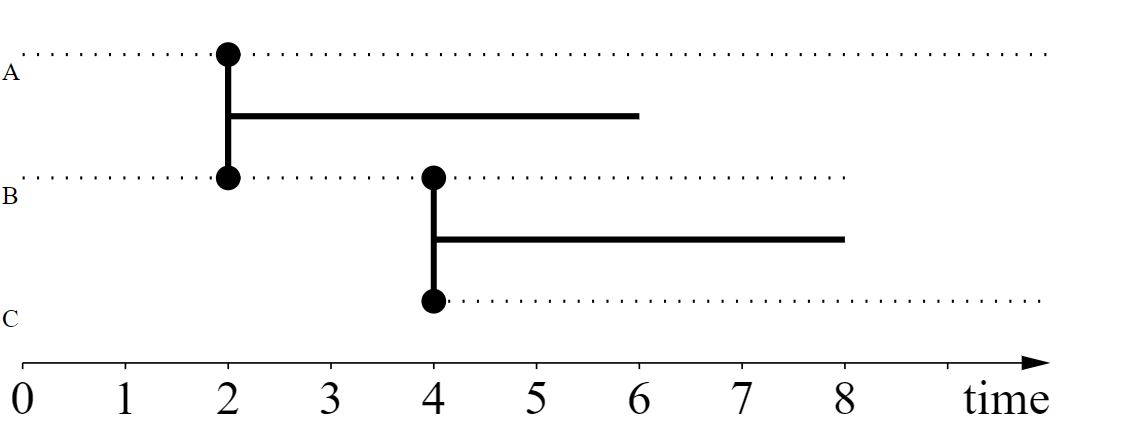
\includegraphics[width=0.5\textwidth]{exStreamGraph.JPG}
\caption{\textbf{Exemple de \stg{} $S=(T,V,W,E)$} Dans cet exemple, on représente les interactions entre des animaux durant une expérience de 10 heures ($T=[0,10]$). Les nœuds sont les trois individus ($V=\{A,B,C\}$), $W=[0,10]\times A \cup [0,8]\times B \cup [0,10]\times C$ représente les moments où les individus étaient présents dans le milieu d'observation. Enfin les liens $E=([2,6]\times (\text{A},\text{B})) \cup ([4,8]\times(\text{B},\text{C}))$ représentent les moments où les individus ont interagi.}
\label{exstreamgraph}
\end{figure}


Dans l'article \cite{stream}, de nombreuses notions sont ensuite définies de telle sorte à ce que dans le cas où le \stg{} serait statique, on retrouve les mêmes notions que pour un graphe classique. Sont ainsi définis, entre autres, le \textit{nombre de n\oe{}uds}, la \textit{densité}, l'\textit{uniformité}, la \textit{compacité}, le \textit{degré}, la \textit{centralité intermédiaire} ainsi que les notions correspondant aux \textit{chemins}, et aux \textit{distances}.

\subsubsection{\Stgs{} et graphes dynamiques}
La notion de \stg{} est très récente (2017)\cite{stream} et ce n'est évidemment pas la première tentative de formalisme pour des graphes dynamiques\cite{temporal}.

Par exemple on peut citer la représentation souvent utilisée en recherche opérationnelle \cite{map,netflow}, en \og snapshot \fg{}. Le nombre de n\oe{}uds d'un système est multiplié par un nombre de pas de temps discrets $n=\frac{t}{T}$. On crée ensuite un graphe temporel dont les n\oe{}uds sont étiquetés $(v,t_i)$, $v$ étant un n\oe{}ud et $t_i$ le temps auquel il est considéré. Les liens peuvent être présents entre différents n\oe{}uds du même pas de temps, et on ajoute à cela une arête entre tous les couples de n\oe{}uds de la forme $(v,t_i),(v,t_{i+1})$. 
Dans ces cas-là les liens sont très souvent orientés pour indiquer le sens du temps. Ces graphes sont utilisés pour des calculs de flots optimaux. On peut d'ailleurs raccrocher cette représentation à la théorie des graphes multicouches, chaque couche correspondant à un pas de temps\cite{mlkiv}. Cependant, cela conduit à avoir des graphes de très grande taille et il faut alors faire un choix entre précision dans le découpage en pas de temps et complexité. Ce choix non trivial, est encore un problème ouvert\cite{dtnontrivial,dtnontrivial2}. De plus, dans les jeux de données réelles, les graphes sont souvent creux et leur représentation matricielle est alors très coûteuse inutilement en mémoire, d'autant plus si on augmente le nombre de pas de temps.


La notion de \stg{} sert à représenter des données d'\textit{interactions}, plus que des données de \textit{relation}. Elle cherche à capturer à la fois leur composante structurelle et temporelle. 

\begin{figure}
\centering
	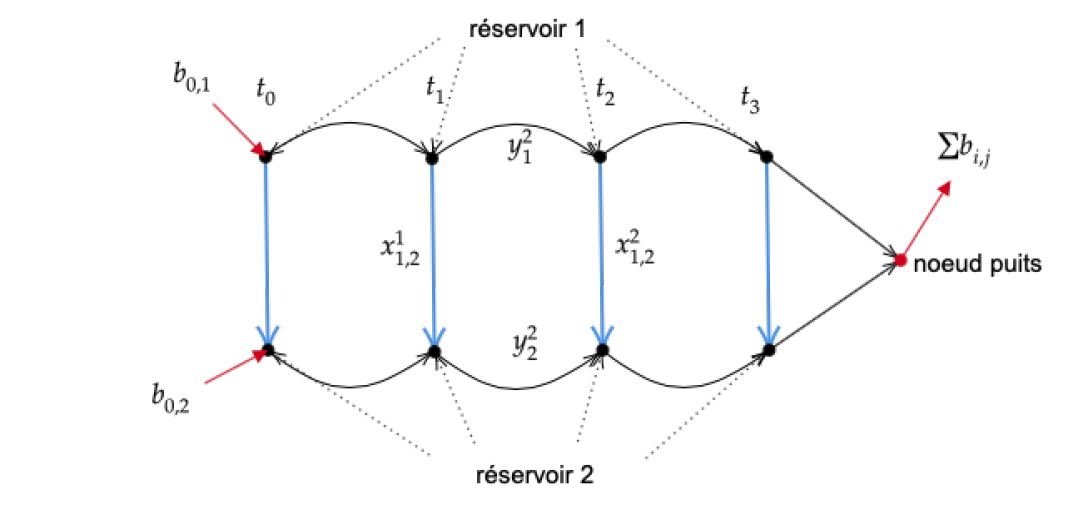
\includegraphics[width=0.7\textwidth]{snapshot.JPG}
	\caption{\textbf{Exemple de snapshot:} Un \og snapshot \fg{} représentant un barrage (liens bleus) entre deux réservoirs aux temps $t_0,t_1,t_2,t_3$, tiré d'un projet MAP552}
\end{figure}



%conclusion partielle : cohérence avec les graphes classiques, à l'utilisateur de choisir ce qu'il veut obtenir



 
\section{Présentation d'un nouvel objet: le \stgm{}}

    Nous avons donc présenté deux formalismes permettant de décrire deux généralisations des graphes. Les \textbf{graphes multicouches} servent à différentier plusieurs types de relations et de n\oe{}uds, qui appartiennent à des catégories discrètes différentes. Les \stgs{} servent à décrire des interactions dépendantes du temps entre divers acteurs, qui peuvent également apparaitre ou non au cours du temps.
    
    
    Notre objectif est de généraliser deux modèles que nous avons présenté pour en pour en créer un nouveau, que nous appelons \textit{\stgm{}}, afin de pouvoir décrire des graphes à structures complexes qui dépendent du temps.
    
    
    En premier lieu, nous définissons de façon formelle cet objet puis nous donnons quelques notions élémentaires, permettant notamment le lien avec les graphes multicouches et les \stgs{}.


\subsection{Définition}

    Un \textbf{\stgm{}}  (ou \textit{multilayer stream graph} en anglais) est un tuple $S_M = (T,T_M,V,W_M,E_M,{\cal L})$.
    
    $T$ est un intervalle de temps, ${\cal L}$ la structure de couches définie comme dans le cadre des graphes multicouches \cref{structure}, et $V$ un ensemble de n\oe{}uds. Une couche est un élément de $L=L_1\times \dots \times L_k$, $\{L_1,\dots L_k\}={\cal L} $.
    
    $T_M=\{T_{\alpha}\subseteq T, \alpha \in L \}$ est un ensemble d'intervalles, indexé par les couches de $L$. Chaque intervalle $T_{\alpha}$ représente le temps d'apparition de la couche $\alpha$, avec pour contrainte que l'ensemble des intervalles d'apparition des couches recouvre $T$: $\cup_{\alpha \in L} T_{\alpha} = T$. 
    
    $W_M \subseteq T \times V \times L$, contient les temps d'existence de chaque nœud-couche, sachant que le temps d'existence d'un nœud-couche est inclus dans le temps d'existence de la couche: si $(t,u,\alpha) \in W_M$, cela signifie que le n\oe{}ud $u$ apparait dans la couche $\alpha$ au temps $t$. Enfin, $E_M \subseteq T \times V \times L \times V \times L$ donne les liens entre les nœuds couches et leurs temps d'existence, sachant qu'un lien ne peut exister que pendant l'intersection des temps d'existence des nœuds-couches qu'il relie.
    
    
    
    On définit également les temps d'existence des n\oe{}uds-couches $T_{u,\alpha}=\{t| (t,u,\alpha) \in W_M \}$ et les temps d'existence des liens $T_{(u,\alpha),(v,\beta)}=\{t| (t,(u,\alpha),(v,\beta)) \in E_M \} $ qui sont des unions d'intervalles.

	
	\begin{figure}[H]
		\centering
		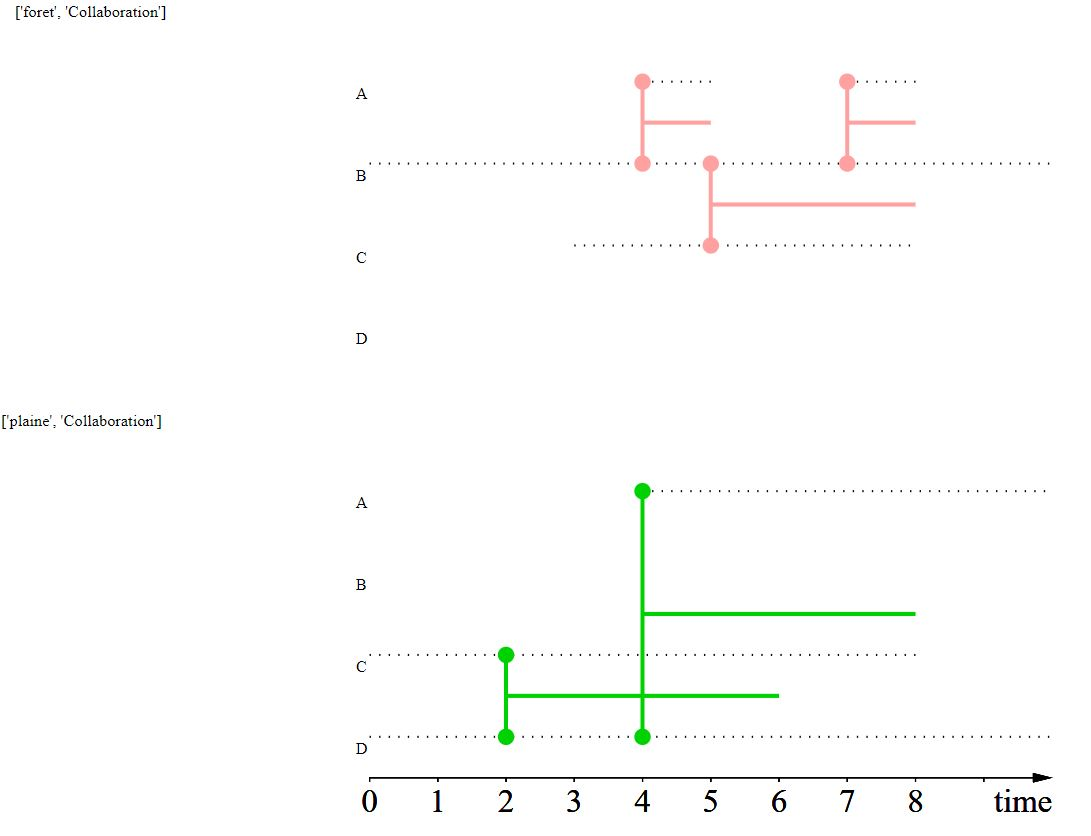
\includegraphics[width=0.8\textwidth]{exMultiStream.JPG}
		\caption{La représentation en \stgm{} des couches \texttt{["plaine","Collaboration"]} et \texttt{["foret","Collaboration"]}, générée avec \og multiplex-stream \fg{} (description du programme en \cref{descode})}
		\label{exstgm}
	\end{figure}
	

\subsection{Extraction de sous-graphes}
\label{sousgraphes}
\subsubsection{Projection par rapport au temps}
	Nous définissons ici deux moyens d'extraire des graphes multicouches induits par un \stgm{}.
	
	Le premier consiste à prendre un instantané au temps $t$ :
	\begin{defn}[Graphe multicouche au temps t]
   	Le {\em graphe multicouche au temps t} $M_t$ s'écrit $M_t = (V_{M,t}, E_{M,t},V,{\cal L})$ avec $V_{M,t}$ et $E_{M,t}$ contenant les n\oe{}uds-couches et les arrêtes apparaissant au temps $t$.
   	$$ V_{M,t} = \{ (u,\alpha) | (t,u,\alpha) \in W_M\} $$
   	$$ E_{M,t} = \{(u,\alpha,v,\beta) | (t,u,\alpha,v,\beta) \in E_M\}$$
    \textit{(Exemple de graphe multicouches au temps $t=4$ et $t=7$ à la \cref{tempst}.)}
   \end{defn}

	\begin{figure}[H]
		\begin{minipage}{0.45\linewidth}
			\captionsetup{margin=10pt}
			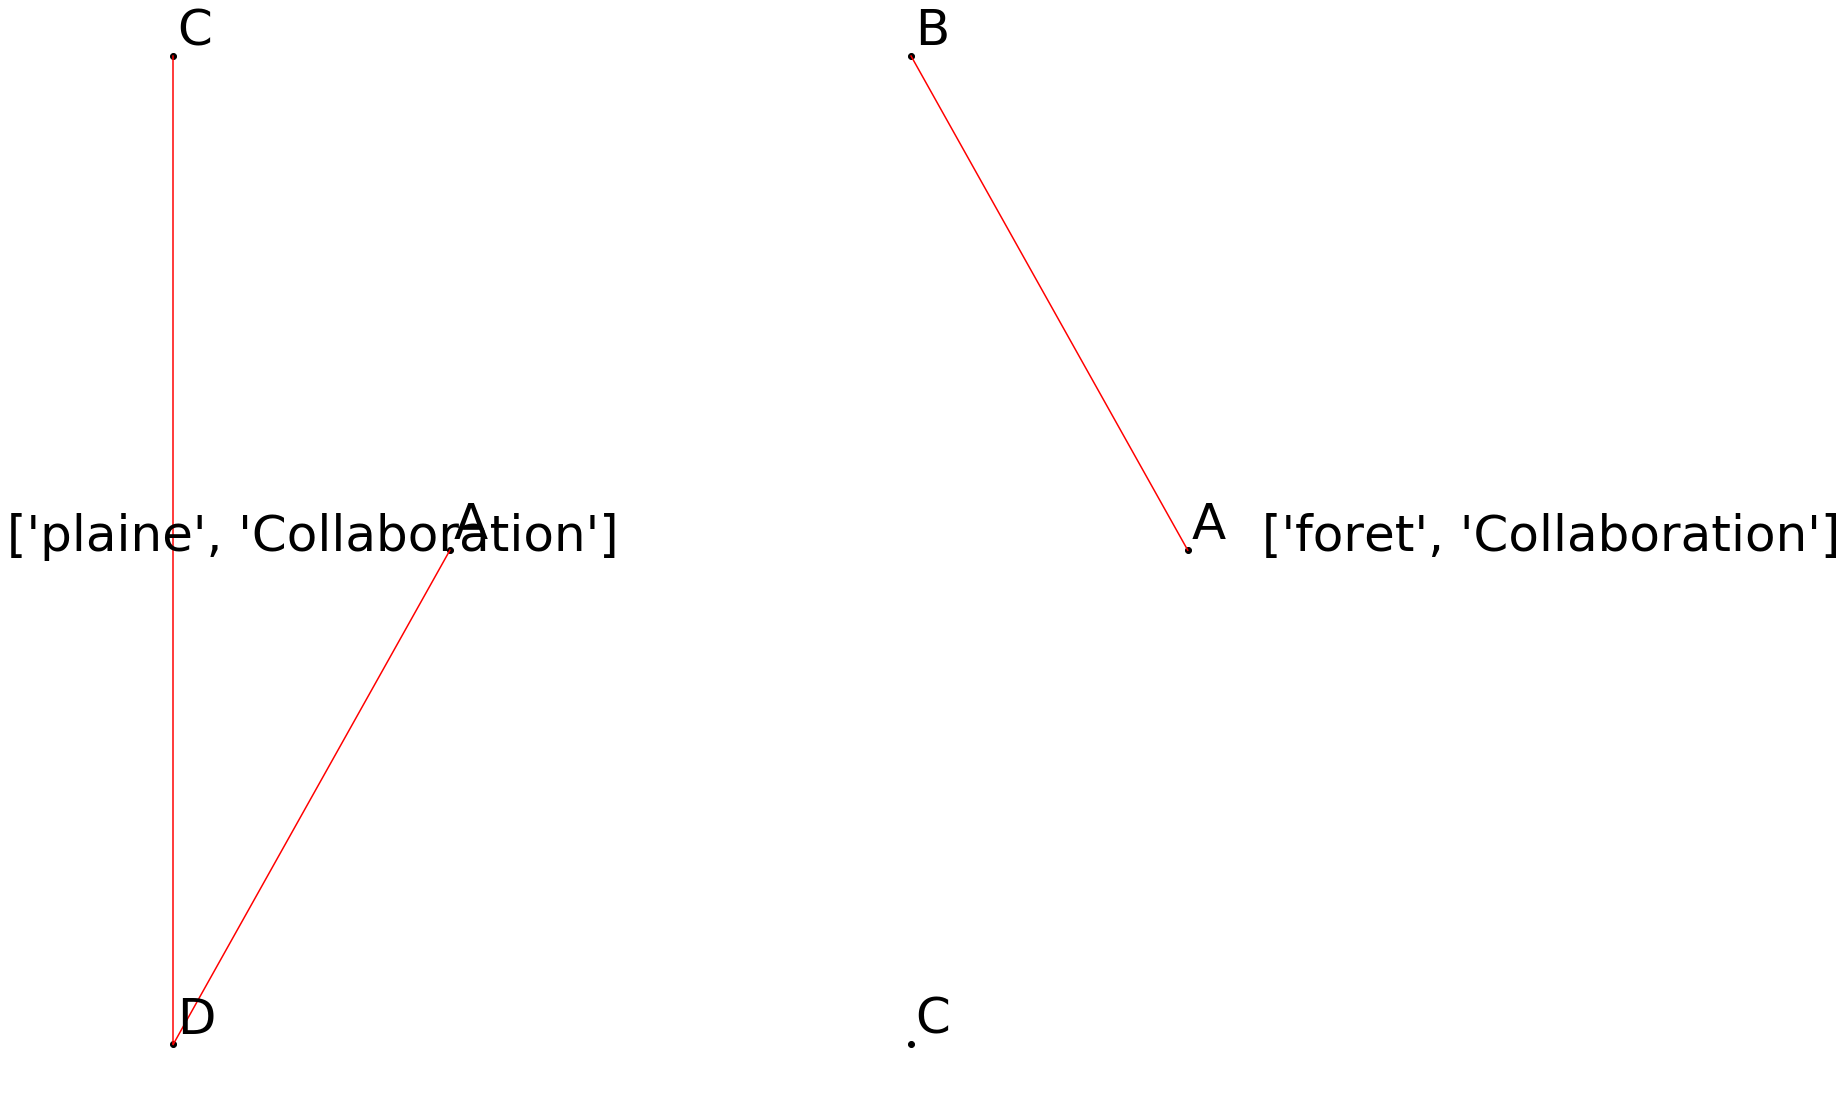
\includegraphics[width=\textwidth]{extrt4ex.png}
			\caption{Extraction du \stgm{} de la \cref{exstgm} au temps $t=4$}
		\end{minipage}
		\begin{minipage}{0.45\linewidth}
			\captionsetup{margin=10pt}
			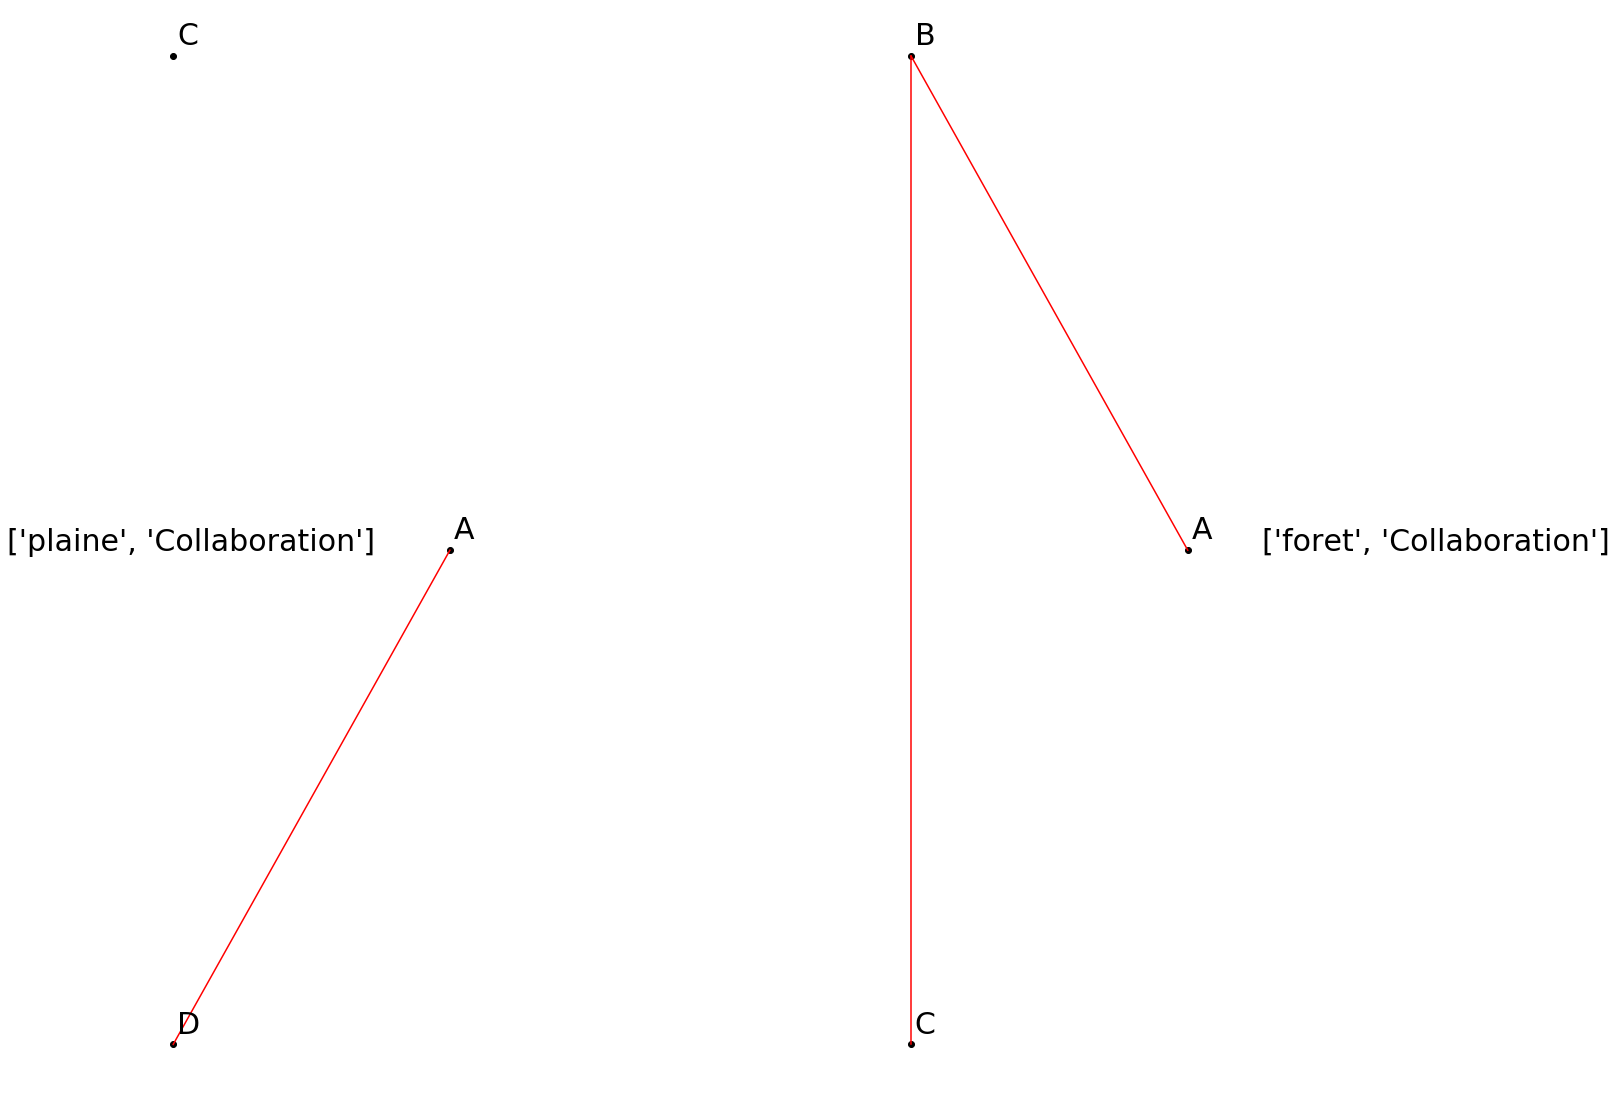
\includegraphics[width=\textwidth]{extrt7ex.png}
			\caption{Extraction du \stgm{} de la \cref{exstgm} au temps $t=7$}
		\end{minipage}
		\caption{Dessin d'une extraction}
		\label{tempst}
	\end{figure}

    Le second consiste à \og enregistrer \fg{} toutes les interactions pendant un laps de temps.
    \begin{defn}[Graphe multicouches induit]
    Le {\em graphe multicouches induit sur l'intervalle $I$} $M_I(S_M) = (V_{M,I}, E_{M,I}, V,L)$ de $S_M$ est le graphe multicouche qui rassemble toutes les couches, n\oe{}uds couches et n\oe{}uds qui apparaissent durant $I$.
    \begin{align*}
    	V_{M,I} = \bigcup_{t\in I} V_{M,t}\\
    	E_{M,I} = \bigcup_{t\in I} E_{M,t}\\
    \end{align*}
    \textit{(Exemple de graphe multicouche induit sur $[0,10]$ à la \cref{induitee})}
    \end{defn}
    
    \begin{figure}[H]
    	\centering
    	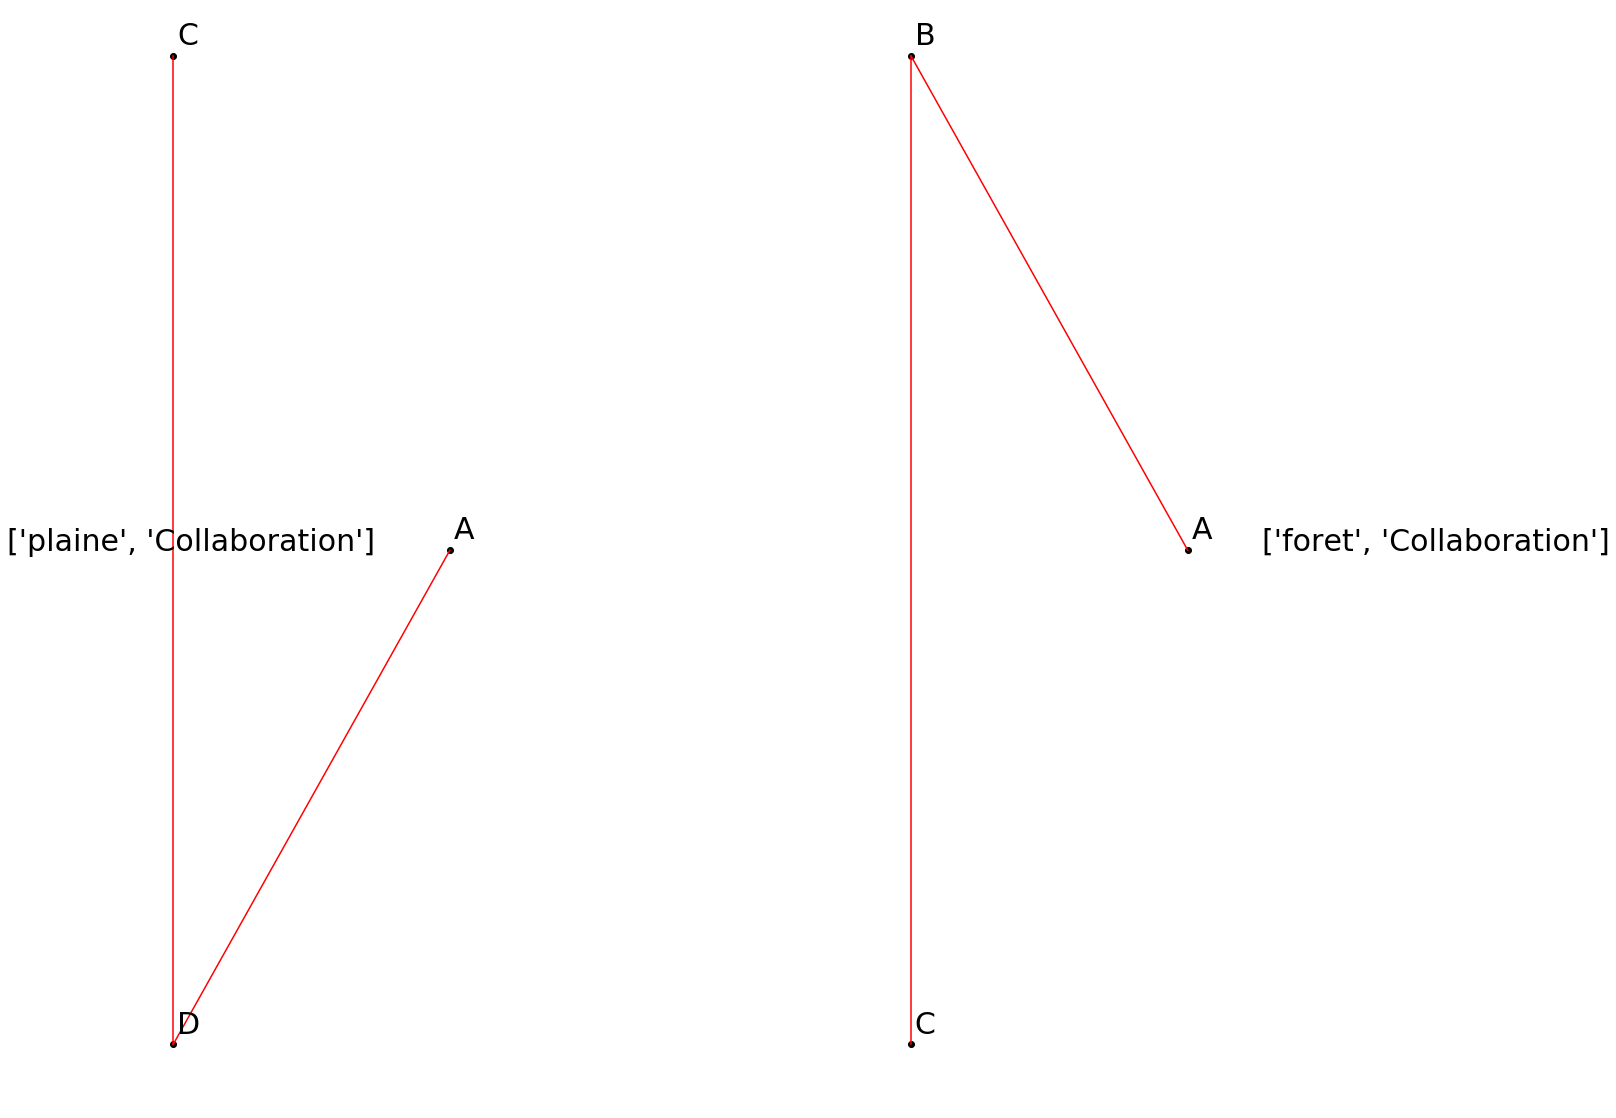
\includegraphics[width=0.5\textwidth]{extrt010.png}
    	\caption{Graphe multicouche induit du \stgm{} de la \cref{exstgm}.}
    	\label{induitee}
    \end{figure}
	


\subsubsection{Projection à partir de couches}
Comme dans l'article de Kivelä\cite{mlkiv} pour les graphes multicouches, nous pouvons classifier les arêtes en plusieurs catégories :
	
	\begin{defn}[Arêtes de couplage, arêtes intra-couches et inter-couches]

   	Les {\em arêtes de couplage} sont définies par l'ensemble $E_C=${\Large\{}$(t,u,\alpha,v,\beta)\in E_M | u=v${\Large\} }.

    Les {\em arêtes intra-couches} sont définies par l'ensemble $E_I = ${\Large\{}$(t,u,\alpha,v,\beta) \in E_M | \alpha = \beta ${\Large\}}.

    Les {\em arêtes inter-couches} sont définies par l'ensemble $\bar{E_I} = E_M\backslash E_I$.
    
	%(See fig.\ref{exIntraInter} for a visual representation.)
	
	\end{defn}	
	
	
	Nous définissons ici de façon formelle les \stgs{} multiplexes.
	
	\begin{defn}[\Stgs{} multiplexe]	
	Un {\em \stg{} multiplexe} $S_{mp}$ est un \stgm{} dans lequel chaque arête est une arête intra-couche ou une arête de couplage. $S_{mp}= (T,T_M,V,W_M,E_M,{\cal L})$ avec $E_M \subseteq \{(t,(u,\alpha),(v,\beta)) | u = v \text{ ou } \alpha=\beta \}$
	\end{defn}
	
	Comme dit précédemment, les graphes multiplexes sont présents dans beaucoup de cas concrets et font l'objet d'études qui leur sont particulièrement dédiées et que nous pouvons adapter aux \stgs{} multiplexes. 

    \vspace{1cm}

	Il peut être intéressant d'extraire certaines couches du \stgm{}, ou au contraire de se focaliser sur des interactions entre couches.
	 
	\begin{defn}[\Stg{} intra-couche]
	Pour chaque couche $\alpha \in L_1 \times \dots \times L_d$, le {\em \stg{} intra-couche} $S^{\alpha}$ est le \stg{} $S^{\alpha}=(T_{\alpha},V^{\alpha},W^{\alpha},E^{\alpha})$ tel que $ T_{\alpha} \in T_M$ est l'intervalle d'existence de $\alpha$. $V^{\alpha}$ est l'ensemble des nœuds couches dans la couche $\alpha$ et $W^{\alpha}$ représente leurs temps d'apparence dans la couche $\alpha$. $E^{\alpha}$ est le sous-ensemble $E_M$ contenant seulement les arêtes entre les n\oe{}uds-couches de $\alpha$.
	\end{defn}
	
	
	\begin{defn}[\Stg{} inter-couches]	
	\'Etant donné un doublet de couches $\alpha, \beta \in L_1\times \dots\times L_d$, le {\em \stg{} inter-couches} est le \stg{} $S^{(\alpha,\beta)} = (T^{\alpha,\beta}, V^{\alpha,\beta},W^{\alpha,\beta},E^{\alpha,\beta})$ tel que : $T^{\alpha,\beta}=T^{\alpha}\cap T^{\beta}$ est l'intervalle durant lequel $\alpha$ et $\beta$ apparaissent simultanément. $V^{\alpha,\beta}$ sont tous les n\oe{}uds-couches du \stgm{} qui sont dans les couches $\alpha$ et $\beta$, $W^{\alpha,\beta}$ décrit leurs intervalles d'existence. Enfin, $E^{\alpha,\beta}$ sont les liens non orientés entre les n\oe{}uds couches des couches de $\alpha$ et $\beta$ avec leurs temps d'existence.
	\end{defn}
	
	%english Notice that for any layer $\alpha$,  is equivalent to $S^{(\alpha,\alpha)}$.

	Pour toute couche $\alpha$, nous définissons $S^{(\alpha)}=S^{(\alpha,\alpha)}$.


	L'étude des opérations d'union et d'intersection permet de trouver des propriétés pertinentes.
	
	\begin{defn}[Intersection de deux \stg{}]
	L'{\em intersection} de deux \stgs{} $S_1$ et $S_2$ est un \stg{} et elle est définie de la façon suivante :
	\[
		S' = S_1 \cap S_2 = (T_1\cap T_2, V_1 \cap V_2, W_1 \cap W_2, E_1\cap E_2)
	\]
	\end{defn}
	

	\begin{defn}[Union de deux \stgs{}]
	L'{\em union} de deux \stgs{} $S_1$ et $S_2$ est un \stg{} et est définie de la façon suivante :
	\[
		S' = S_1 \cup S_2 = (T', V_1 \cup V_2, W_1 \cup W_2, E' \})
	\]
	$T'$ est un intervalle :
	\[
		T' = [\min(T_1,T_2),\max(T_1,T_2)]
	\]
	\[
		E' = E_1 \cup E_2 
	\]
	
	\end{defn}
	
	

	
	\begin{defn}[\Stg{} sous-jacent]
	Le {\em \stg{} sous-jacent} $S_U(S_M)$ de $S_M$ est $(T,V_M,W_M,E_M)$. C'est un \stg{} dans lequel les n\oe{}uds sont les n\oe{}uds-couches de $S_M$. Il peut être partitionné selon les différentes couches.
	\end{defn}
	
	\begin{defn}[\Stg{} agrégé]
		Le {\em \stg{} agrégé} $S_A(S_M)=(T,V,W_A,E_A)$ a le même intervalle d'étude $T$ que $S_M$. Ses n\oe{}uds sont l'ensemble $V$ de ceux de $S_M$. Leurs temps d'existences sont l'union de leurs temps d'existences sur les différentes couches: $T_u = \bigcup_{\alpha \in L} T_{u,\alpha}$ et $W_A=\bigcup_{u\in V} T_u\times\{u\}$. Une arête existe entre deux n\oe{}uds de $S_A(S_M)$ si elle existe au même temps entre deux n\oe{}uds-couches correspondants de $S_M$: $E_A = \{(t,u,v)| \exists (\alpha,\beta) \in L^2, (t,(u,\alpha),(v,\beta)) \in E_M \}$
	\end{defn}
	
	Nous démontrons que le \stg{} sous-jacent $S_U(S_M)$ est égal à l'union de tous les \stg{} inter et intra couches.
	
		
	\begin{prop}
		\[
			\bigcup_{(\alpha,\beta) \in L^2} S^{(\alpha,\beta)} = S_U(S_M)
		\]
	\end{prop}
	\begin{proof}
	On appelle $S=\bigcup_{(\alpha,\beta) \in L^2} S^{(\alpha,\beta)}=(T^{*},V^{*},W^{*},E^{*})$. Montrons que $S=S_U(M_S)= (T_U,V_U,W_U,E_U)$.
	
	$T=T_U$ par définition de $S_U$. Par construction des \stgms{}, pour tout $t$ dans $T$, il existe au moins une couche $\alpha$. Comme $T^* = [\min_{\alpha \in L} (T^{\alpha}),\max_{\alpha \in L} (T^{\alpha})]$, $t$ est forcément inclus dans $T^*$. Chaque $T^{\alpha}$ est inclus dans $T$, donc $T^* \subseteq T$, donc $T^*=T_U=T$.
	
	$V_M = V_U$ par définition de $V_U$.$V^{*}=\bigcup_{(\alpha,\beta) \in L^2} V^{\alpha,\beta} \subseteq V_M$. Tous les n\oe{}uds de toutes les couches sont inclues dans $\bigcup_{(\alpha) \in L^2} V^{\alpha,\alpha} \subseteq V^{*}$, on obtient donc l'égalité $V_M=V_U=V^*$.
	Avec le même raisonnement, nous trouvons $W_M=W_U=W^*$.
	
	$E_U=E_M$ et $E^{*}=\bigcup_{\alpha,\beta \in L^2}(E^{\alpha,\beta})$ par définition. Comme $E^{\alpha,\beta}$ est un sous-ensemble de $E_M$ pour chaque couple de couches $\alpha,\beta$, $E^{*} \subset E_M$. On sait également que pour toute arête $e =(t,u,\alpha,v,\beta) \in E_M$, $e$ appartient à $E^{\alpha,\beta}$. Donc $E_M=E^{*}$.


On a donc bien une égalité terme à terme entre tous les éléments de $S$ et de $S_U(M_S)$.					
	\end{proof}


Nous avons donc exhibé un certain nombre d'extractions que nous pourrons maintenant combiner pour obtenir des graphes, des \stg{} ou des graphes multiplexes, en fonction des résultats que nous voudrons obtenir.

\subsection{Mesures}


Nous avons créé des mesures permettant de mesurer la présence de liens et de nœuds dans les graphes. Nous voulons que ces mesures soient adaptées à l'objet spécifique que nous étudions (et qu'elles prennent en compte l'aspect multicouche et l'aspect temporel de façon simultanée), qu'elles aient des noms qui évoquent intuitivement ce qu'elles expriment et que chacune soit une généralisation des notions utilisées pour les \stgs{}, pour les graphes multicouches et pour les graphes.

	\subsubsection{Nombre de nœuds et nombre de liens}
	Le {\em nombre de n\oe{}uds dans un graphe} $G=(V,E)$ est $n=|V|$ et le nombre d'arêtes est $m=|E|$.
	
	Le {\em nombre de n\oe{}uds dans un \stg{}} $S=(T,V,W,E)$ est défini dans \cite{stream} comme $\hat{N}^T_n=\frac{|W|}{|T|}=\sum_{v\in V} n_v$ (ce qui est en fait le nombre moyen de n\oe{}uds au cours du temps). $n_v$ est appelé {\em contribution de v} et est égal à $\hat{N}^T_v=\frac{|T_v|}{|T|}$. Remarquons bien qu'ici cette notion est différente {\em du nombre de n\oe{}uds dans} $|V|$, sauf quand le \stg{} $S$ est constant au cours du temps.
	\newline
	
	Dans les graphes multicouches, une telle notion n'a pas été définie explicitement.
	Nous avons donc défini le {\em nombre moyen de n\oe{}uds par couche} comme :
	\begin{align*}
		\hat{N}_n^L(M_l) = \frac{\text{nombre de n\oe{}ud-couches}}{\text{nombre de couches}}=\frac{|V_M|}{|L|}
	\end{align*}	    
	Remarquons que dans le cas d'un monocouche, nous retrouvons le nombre de n\oe{}uds classique, ce qui signifie que nous pouvons choisir cette mesure comme une généralisation du {\em nombre de nœuds} dans un graphe, comme cela a été fait dans \cite{stream} pour les \stg{}.
		
	
	\begin{defn}[Contribution des couches]
	On définit la {\em contribution} d'une couche comme suit : $n_\alpha = \frac{|T_{\alpha}|}{|T|}$. Le {\em nombre de couches dans un \stgm{}} est la somme des contributions. $$\hat{N}^T_l = \sum_{\alpha \in L}\frac{ |T_{\alpha}|}{|T|}$$.
    \end{defn}
	
	\begin{defn}[Contribution et quantité de nœud-couches]
	La {\em contribution d'un n\oe{}ud-couche} $(v,\alpha)$ dans un \stgm{} est $n_{v,\alpha} = \frac{|T_{v,\alpha}|}{|T|}$. Le {\em nombre de nœud-couches} est la somme de leurs contributions $\hat{N}^{T}_{nl}(M) = \underset{(u,\alpha)\in V_M}{\sum} n_{u,\alpha} = \frac{|W_M|}{|T|}$.
    \end{defn}
	
	Dans le cas d'un \stg{} monocouche, nous retrouvons bien que le nombre de n\oe{}uds est égal au nombre de n\oe{}uds-couches. En prenant le \stg{} sous-jacent du \stgm{}, on retrouve également que le nombre de n\oe{}uds est égal au nombre de n\oe{}uds couches. Nous avons donc là une généralisation satisfaisante du nombre de n\oe{}uds-couches.
    
   Enfin, nous définissons le \textbf{nombre de n\oe{}uds et de liens dans un \stgm{}} de la façon suivante : 
    
    \begin{defn}[Contribution et nombre de n\oe{}uds dans un \stgm{}]
    La {\em contribution} d'un n\oe{}ud décrit le taux d'apparition d'un n\oe{}ud dans les couches : $n_v = \frac{\sum_{\alpha \in L}|T_{v,\alpha}|}{\sum_{\alpha \in L} |T_{\alpha}|}$.
    
    Le {\em nombre de n\oe{}uds} est la somme de ces contributions:
    \[
    \hat{N}^{L,T}_n(M) = \sum_{v\in V} n_v=\sum_{v\in V} \frac{\sum_{\alpha \in L}|T_{v,\alpha}|}{\sum_{\alpha \in L} |T_{\alpha}|} =\frac{1}{{\sum_{\alpha \in L} |T_{\alpha}|}}\sum_{v\in V} \sum_{\alpha \in L}|T_{v,\alpha}|
    \]
	
	\end{defn}
	
	Cette définition est cohérente avec les notions des multicouches et des \stg{} : si le n\oe{}ud apparait dans toutes les couches tout le temps, nous trouvons $n_v=1$ comme dans les multicouches. Si tous les temps d'existence sont égaux, on retrouve $$n_v=\frac{|\{(u,\alpha) \in V_M | u=v \}|  \times |T|}{|L|\times |T|}$$
	
	\begin{defn}[Nombre de liens dans un \stgm{}]
	    Le nombre de lien dans un \stgm{} se calcule comme le nombre de liens dans un \stg{}. $$n_l=\frac{\sum_{(u,\alpha)(v,\beta)\in E_M}|T_{(u,\alpha)(v,\beta)}|}{|T|}$$
	\end{defn}
	


	


	\subsubsection{Uniformité et densité}
	
	Dans les \stgs{} \cite{stream}, {\em l'uniformité entre deux nœuds} $u$ et $v$ est le ratio $\Cup (u,v) = \frac{|T_u\cap T_v|}{|T_u \cup T_v|}$, c'est à dire la probabilité, prenant un temps $t$ dans $T_u\cup T_v$, que les deux nœuds $u$ et $v$ puissent être reliés entre eux. L'uniformité est définie comme le rapport de tous les temps de co-existence sur les temps d'existence : $
 \Cup(S)=\sum_{u,v \in V \otimes V}\frac{|T_u\cap T_v|}{|T_u\cup T_v|}
$
	
		
	{\em L'uniformité } de deux n\oe{}uds-couches $(u,\alpha)$ et $(v,\beta)$ est définie sur le même modèle:
	\begin{align*}
		\Cup((u,\alpha),(v,\beta)) &=\mathbb{P}( t \in T_{u,\alpha} \cap T_{v,\beta} | t \in T_{u,\alpha} \cup T_{u,\beta}) \\
		&= \frac{|T_{u,\alpha}\cap T_{u,\beta}|}{|T_{u,\alpha}\cup T_{u,\beta}|}
	\end{align*}

	{\em Le chevauchement} de deux couches $\alpha$ et $\beta$ est également défini comme suit:
	\begin{align*}
		\Cup(\alpha,\beta) = \frac{|T_{\alpha}\cap T_{\beta}|}{|T_{\alpha}\cup T_{\beta}|}
	\end{align*}

    L'{\em uniformité des n\oe{}uds-couches} mesure le taux d'apparition simultanée des n\oe{}uds-couches dans le \stgm{}:
    \[
    	\Cup(M) = \frac{\sum_{(u,\alpha),(v,\beta) \ V_M \otimes V_M}{|T_{(u,\alpha)} \cap T_{(v,\beta)}|}}{\sum_{(u,\alpha),(v,\beta) \ V_M \otimes V_M}{|T_{(u,\alpha)}\cup T_{(v,\beta)}|}}
    \]
	
	Cette définition peut être nuancée en considérant que selon la nature du \stgm{}, certains n\oe{}uds peuvent ou ne peuvent pas apparaître simultanément. En particulier, {\em l'uniformité dans un \stgm{}} est définie ainsi:	
	
	\[
    	\Cup(M) = \frac{1}{|L|}\sum_{\alpha \in L} \frac{\sum_{(u,\alpha),(v,\alpha) \ V_M \otimes V_M}{|T_{(u,\alpha)} \cap T_{(v,\alpha)}|}}{\sum_{(u,\alpha),(v,\alpha) \ V_M \otimes V_M}{|T_{(u,\alpha)}\cup T_{(v,\alpha)}|}}
    \]
    
    On ne prend en compte que les temps d'apparition intra-couche, et on moyenne selon le nombre de couche. 


	Quand $\Cup=1$, on dit que le \stg{} est \textbf{uniforme} (autrement dit, $T_v = T_u, \forall (u,v) \in V^2$).


    Après avoir mesuré \og à quel point le \stgm{} peut être connecté\fg{} grâce à l'uniformité, nous allons mesurer à quel point il est effectivement connecté grâce à la notion de \textbf{densité}.
    
    Dans les graphes classiques (non pondérés et non dirigés), la {\em densité} est la probabilité, prenant deux n\oe{}uds au hasard dans le graphe, qu'une arête existe entre ces n\oe{}uds.
    
		\[
			d(G) = \frac{|E|}{|V\otimes V|} = \frac{2\times |E|}{|V|(|V|-1)}
		\]
	Dans les \stg{} \cite{stream}, l'intuition est la même, en prenant un temps aléatoire, et deux n\oe{}uds au hasard existant à ce temps. 	

		\begin{align*}
			\delta_s(G) = & \mathbb{P}((t,u,v)\in E| (t,u),(t,v) \in W) \\
			 =  & \frac{\sum_{(u,v) \in V \otimes V}{|T_{uv}|}}{\sum_{(u,v) \in V\otimes V}{|T_u\cap T_v|}}
			 %= \frac{\int_{t\in T}{|E_t|dt}}{\int_{t\in T}{|V_t\otimes V_t|dt}}
		\end{align*}
		
	Nous pouvons ensuite définir la densité dans les \stgms{}. Nous remarquons premièrement que la densité mesure le \og taux de connectivité \fg{}, et qu'une fois encore, en fonction du système étudié, la définition peut changer puisque nous voulons que le cas où la densité est égale à 1 corresponde au cas où on ne peut pas rajouter d'arêtes. 

\begin{defn}[Densité d'un \stgm{}]	
	Nous appelons  $C \in T \times V_M\times V_M$ l'ensemble des liens autorisés dans le \stgm{}. Si certaines liens sont \og automatiques\fg{} ou \og sous-entendus \fg{} comme par exemple les arêtes de couplage, nous ne les comptons pas dans $C$ non plus pour que le cas où la densité soit nulle corresponde au cas où on ne peut pas retirer de lien.

	La {\em densité du \stgm{}} s'écrit alors : 
	\[
		\delta_M (M) 
		%= \frac{\int_{t\in T}|E_M,t|}{\int_{t\in T}|C_t|} 
		= \frac{\sum_{(u,\alpha)(v,\beta) \in E_M}|T_{(u,\alpha)(v,\beta)}|}{|C|}
	\]
\end{defn}	
	
	Par exemple, dans un \stg{} multiplexe, les liens possibles sont les liens intra couches et les liens de couplage: $C=${\Large \{}$(t,u,\alpha),(t,v,\beta))| t\in T_{u,\alpha} \cap T_{u,\beta}, u=v \text{ ou } \alpha = \beta)${\Large \}}:

	\[
		\delta_M (M) = 
		\frac{|E_M|}{|C|}= 
		\frac{\sum_{(u,\alpha)(v,\beta) \in (V_M \otimes V_M)} |T_{(u,\alpha)(v,\beta)}|}
		{\underbrace{\bigg(\sum_{\alpha \in L}\sum_{(u,v) \in V\otimes V}|T_{u,\alpha} \cap T_{v,\alpha}|\bigg)}_{\text{arêtes intra-couches}}+\underbrace{\bigg( \sum_{u \in V } \sum_{(\alpha,\beta) \in L \otimes L}|T_{u,\alpha}\cap T_{u,\beta}|\bigg)}_{\text{arêtes de couplage}}}
	\]


\paragraph{}
Nous avons donc présenté les bases mathématiques des \stgms{}, ayant pour but de représenter des interactions de différentes natures, entre différents acteurs, en fonction du temps. Les mesures de nombre de n\oe{}uds et de liens, d'uniformité et de densité permettent d'adapter des notions présentes dans les graphes à notre objet. Les outils d'extraction comme le graphe sous-jacent, le graphe agrégé ou les sous \stg{} inter et intra-couches permettent de \og retrouver \fg{} les graphes classiques auxquels nous sommes habitués.
	
\section{Application à des données concrètes}
\label{application}

Nous avons ensuite construit une bibliothèque Python \cite{github} pour mettre en application les notions théoriques que nous avons présentées.

Nous présentons cette bibliothèque ainsi que sa structure. Puis, en utilisant un jeu de données approprié, nous donnons un exemple d'utilisation concrète de la bibliothèque et des notions créées.


\subsection{Structure de données et organisation du code} 

\label{descode}

	La gestion des \stgms{} implique assez rapidement de gérer un grand nombre d'informations \og imbriquées \fg{}: chaque couche contient des n\oe{}uds, qui apparaissent à des temps précis, ces n\oe{}ud-couches sont reliés par des liens, eux-mêmes apparaissant dans des intervalles de temps qu'il faut stocker.
	
	Nous choisissons de construire des classes Python pour simplifier la gestion de telles données, et pour permettre de vérifier simplement que le \stgm{} reste cohérent quand on le modifie.
	
	
	
	\begin{figure}[H]
		\centering
		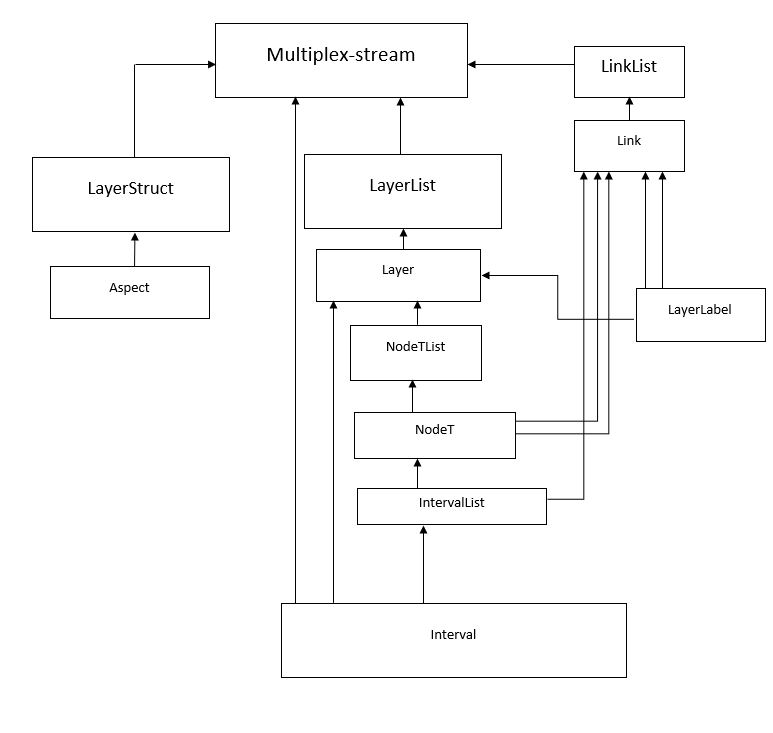
\includegraphics[width=0.7\textwidth]{codeStructure.JPG}
		\caption{Structure du code en classes }
	\end{figure}
	
	Toutes les listes sont toujours triées et les listes d'intervalles contiennent seulement des intervalles disjoints (quitte à fusionner certains intervalles).
	
	Dans un graphe classique, la {\em taille}, c'est à dire le nombre d'éléments à parcourir dans le graphe, est donnée par $c_G(G)=|V|+|E|$. Ici, nous avons choisi de stocker des couches, elles-mêmes contenant les n\oe{}uds-couches (et un intervalle), qui contiennent des listes d'intervalles. Les liens sont caractérisés par deux n\oe{}uds-couches et une liste d'intervalle.
	
	On appelle $n_I$ le nombre d'intervalle d'un ensemble, si celui-ci contient une liste d'intervalles.
	
	Ici la taille du \stgm{} est donc : $c_{MS}(M_S)=\sum_{e \in E_M} n_I(e) + \sum_{\alpha \in L} \sum_{v \in V} n_I((v,\alpha))$. Notons que dans le cas où le \stgm{} est statique et monocouche, on retrouve la taille d'un graphe classique.
	
	Pour traiter de graphes classiques, nous avons généralement le choix entre utiliser une matrice d'adjacence (ce qui nous permet de savoir s'il existe un lien entre deux n\oe{}uds en temps constant) ou d'utiliser des listes d'adjacence (ce qui permet d'économiser de la mémoire).
	
	Ici, le stockage d'un lien est beaucoup plus coûteux puisqu'il faut stocker tous les intervalles d'existence, nous avons plutôt choisi d'utiliser une liste simple de tous les liens, mais stockés de façon ordonnés grâce à la bibliothèque \texttt{sorted collection}, qui permet de retrouver ou d'insérer des éléments par dichotomie (complexité logarithmique).
	

\subsection{CPGE : interactions entre élèves d'un même établissement}

    Nous avons en premier lieu testé notre logiciel avec une jeu de données issu de SocioPatterns~\cite{cpge}, recensant les interactions \og face à face\fg{} entre élèves (enregistrées pendant 5 jours toutes les 20 secondes grâce à des capteurs de proximité), leurs amitiés sur Facebook, et leurs réponses à un questionnaire leur demandant s'ils étaient amis.

    Nous avons donc choisi une structure de couches suivante: \\
    \hspace*{2cm}{\tt L=[type de relation,classe,sexe]},\\
     \hspace*{3cm}avec\\
     \hspace*{2cm}{\tt type de relation = [face to face, facebook, contact, amitié]},\\
     \hspace*{2cm}{\tt classe = "MP","MP*1","MP*2","2BIO1","2BIO2","2BIO3","PSI*","PC","PC*"}.
    
    Comme les seules interactions dépendantes du temps sont celles de face à face, on peut dire que le jeu de données donne lieu à un graphe \og hybride \fg{}. Nous avons considéré que les liens Facebook et d'amitié étaient donc constants au cours du temps.
  
	\subsubsection{Représentation graphique}  
  
  Nous avons tout d'abord tenté de représenter le \stgm{} en entier (\cref{lyceeentier}). La taille du jeu de données le rend difficile à représenter du fait que beaucoup de liens s'entrecroisent. (D'ailleurs, trouver un ordre optimal pour les n\oe{}uds qui limite les croisements des liens avec d'autres n\oe{}uds est un problème d'optimisation en cours de résolution).
  
  Cependant, grâce à une coloration des liens intercouches, nous pouvons tout de même saisir la structure générale du jeu de données, ainsi que les pauses et les nuits.
	
	\begin{figure}[h]
	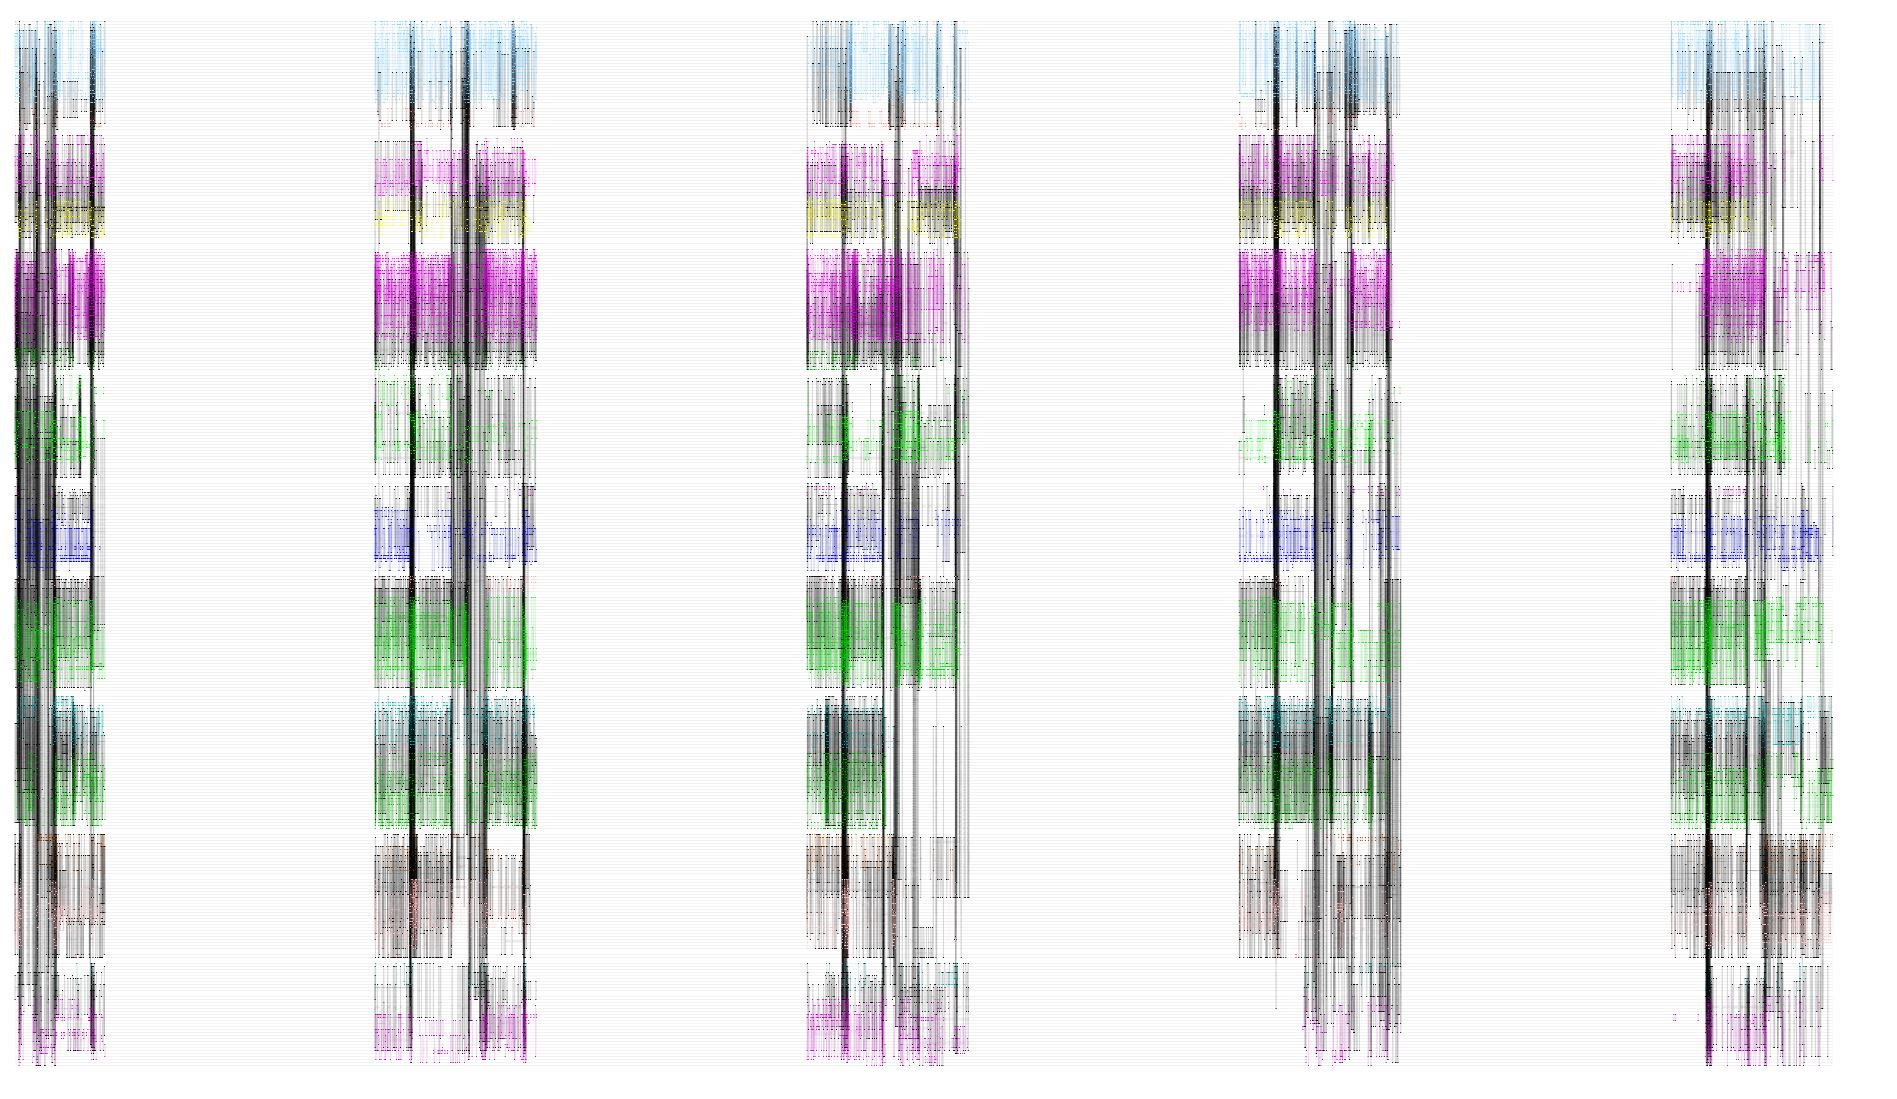
\includegraphics[width=\textwidth]{lyceeentier.JPG}
	\caption{\textbf{Visualisation du \stgm{} du dataset \cite{cpge}.} Les liens intra-couches ont été coloriés dans des couleurs aléatoires pour chaque couche. On remarque des apparitions de liens inter-couches assez importants au moment des \og pauses \fg{} (il y a visiblement une pause le matin, une autre le midi, et une à la fin de la journée). On peut également visualiser simplement l'emploi du temps des élèves (représenté par des vides et des pleins dans le graphe).}
	\label{lyceeentier}
\end{figure}





\subsubsection{Sous-graphes, sous \stg{} et sous graphes multicouches}

Voici quelques exemples de sous-graphes tels que nous les avons définis \cref{sousgraphes}. Nous avons décidé de nous cantonner aux relations \texttt{"face to face"} et \texttt{"facebook"}, mais ces résultats sont généralisables à plus de couches.

\paragraph{Graphe multicouche induit}
	Le graphe multicouche induit des relations de deux classes, filles et garçons, est représenté par la \cref{completinduit}. Ici, chaque cercle de n\oe{}uds (représentés par les points noirs) correspond à une couche différente.
	
\begin{figure}[H]
	\centering
	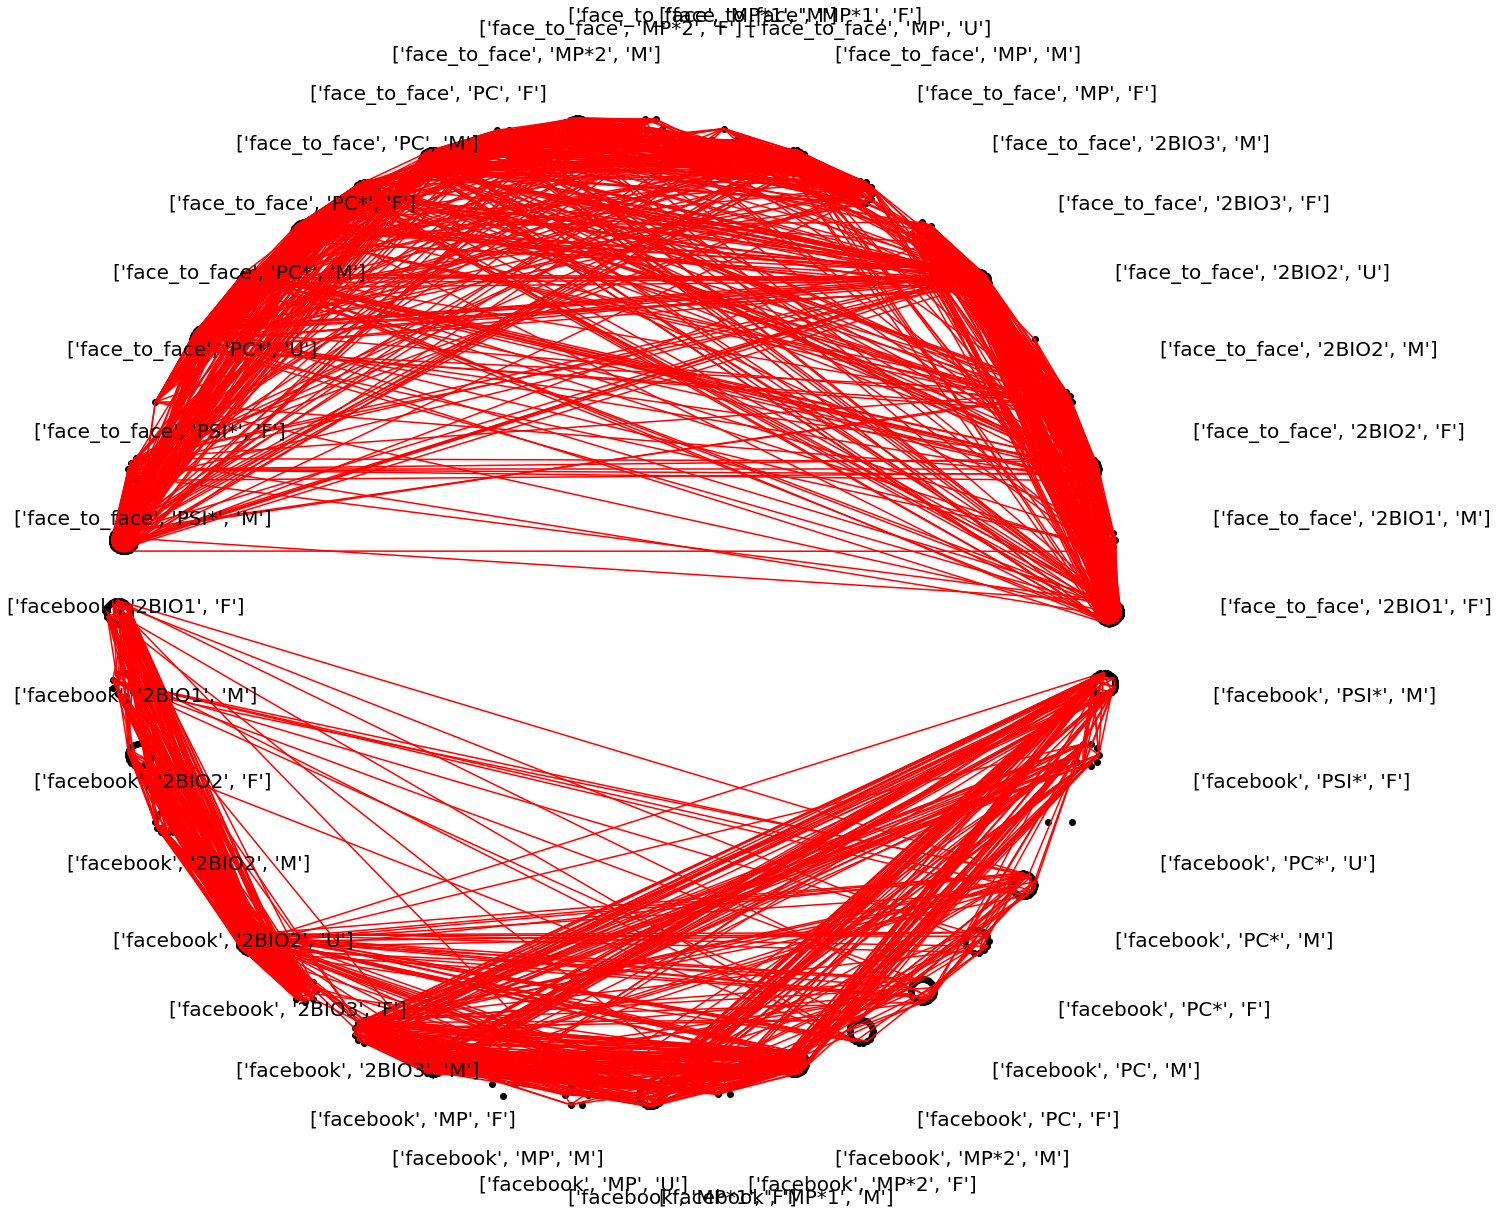
\includegraphics[width=0.5\textwidth]{tout.png}
	\caption{\textbf{Graphe induit}}
	\label{completinduit}
\end{figure}

	Nous représentons ensuite les sous-graphes multicouches intra-couches et inter-couches induits des couches de deux classes différentes pour plus de visibilité dans la \cref{induit}.

\begin{figure}[H]
	\begin{minipage}[t]{0.48\textwidth}
		\captionsetup{margin=10pt}
		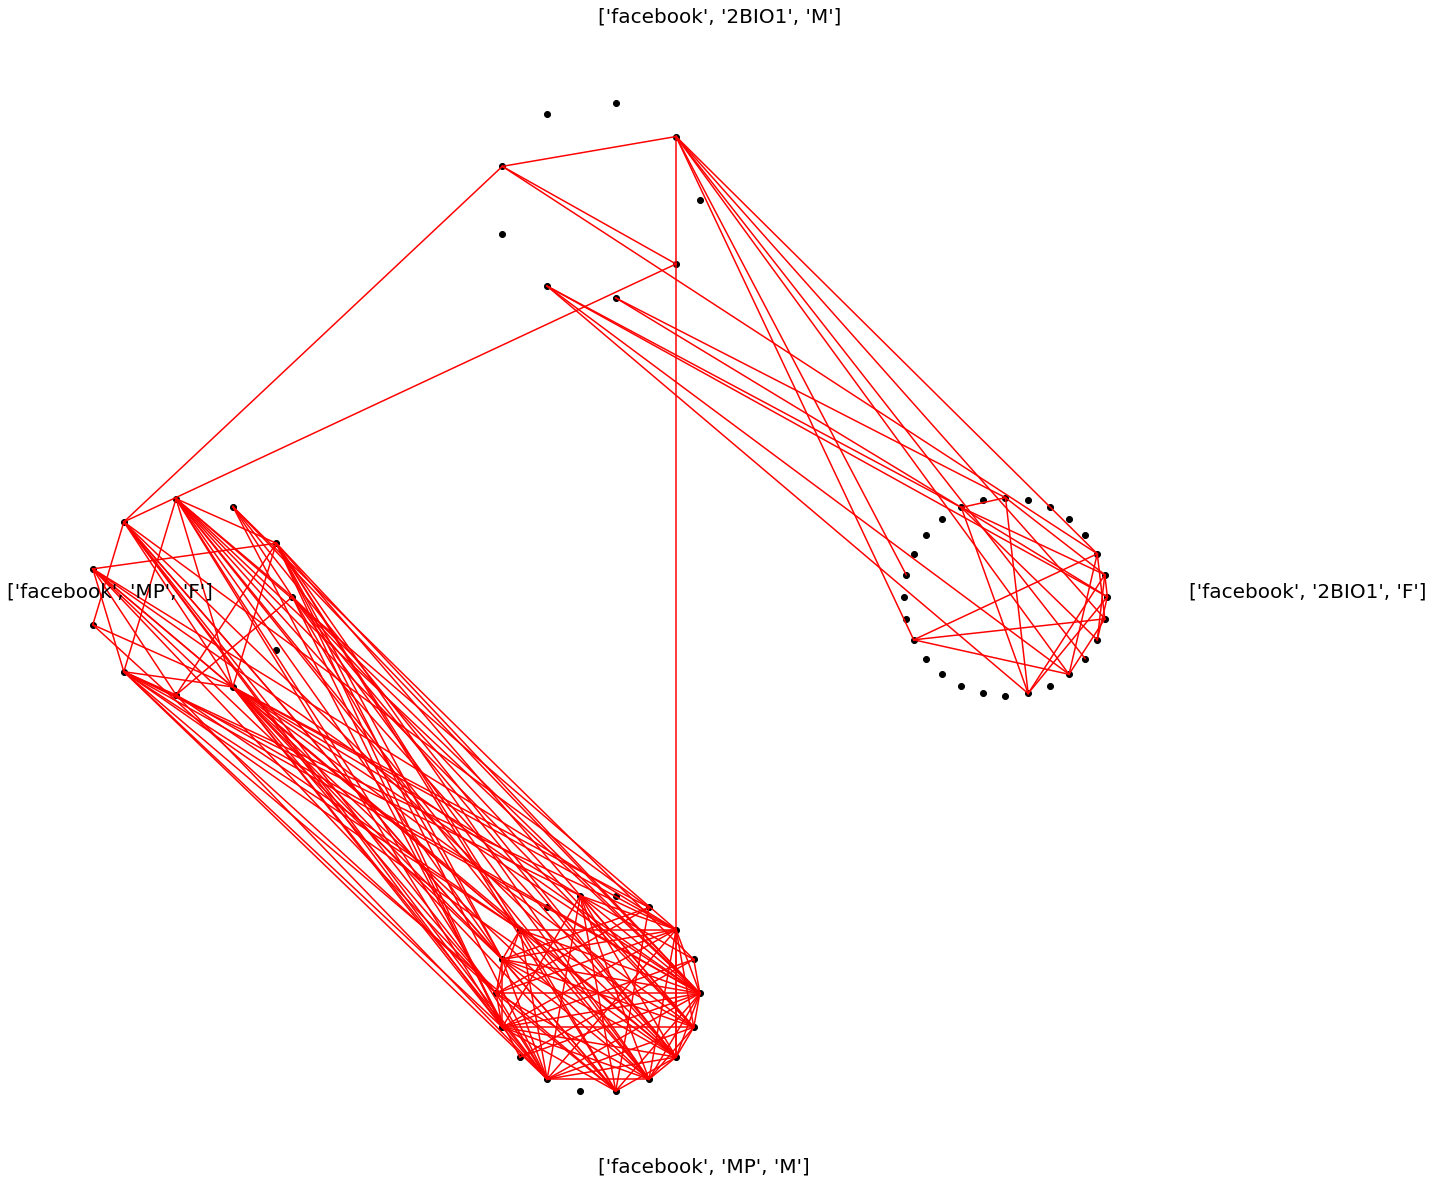
\includegraphics[width=\textwidth]{sousmulticlasse.png}
	\caption{\textbf{Visualisation du sous graphe multicouches des relations \texttt{`facebook'}, entre les élèves de deux classes} : les \texttt{`2BIO1'} et les \texttt{`MP'}.}
	\end{minipage}
	\begin{minipage}[t]{0.48\textwidth}
		\centering
		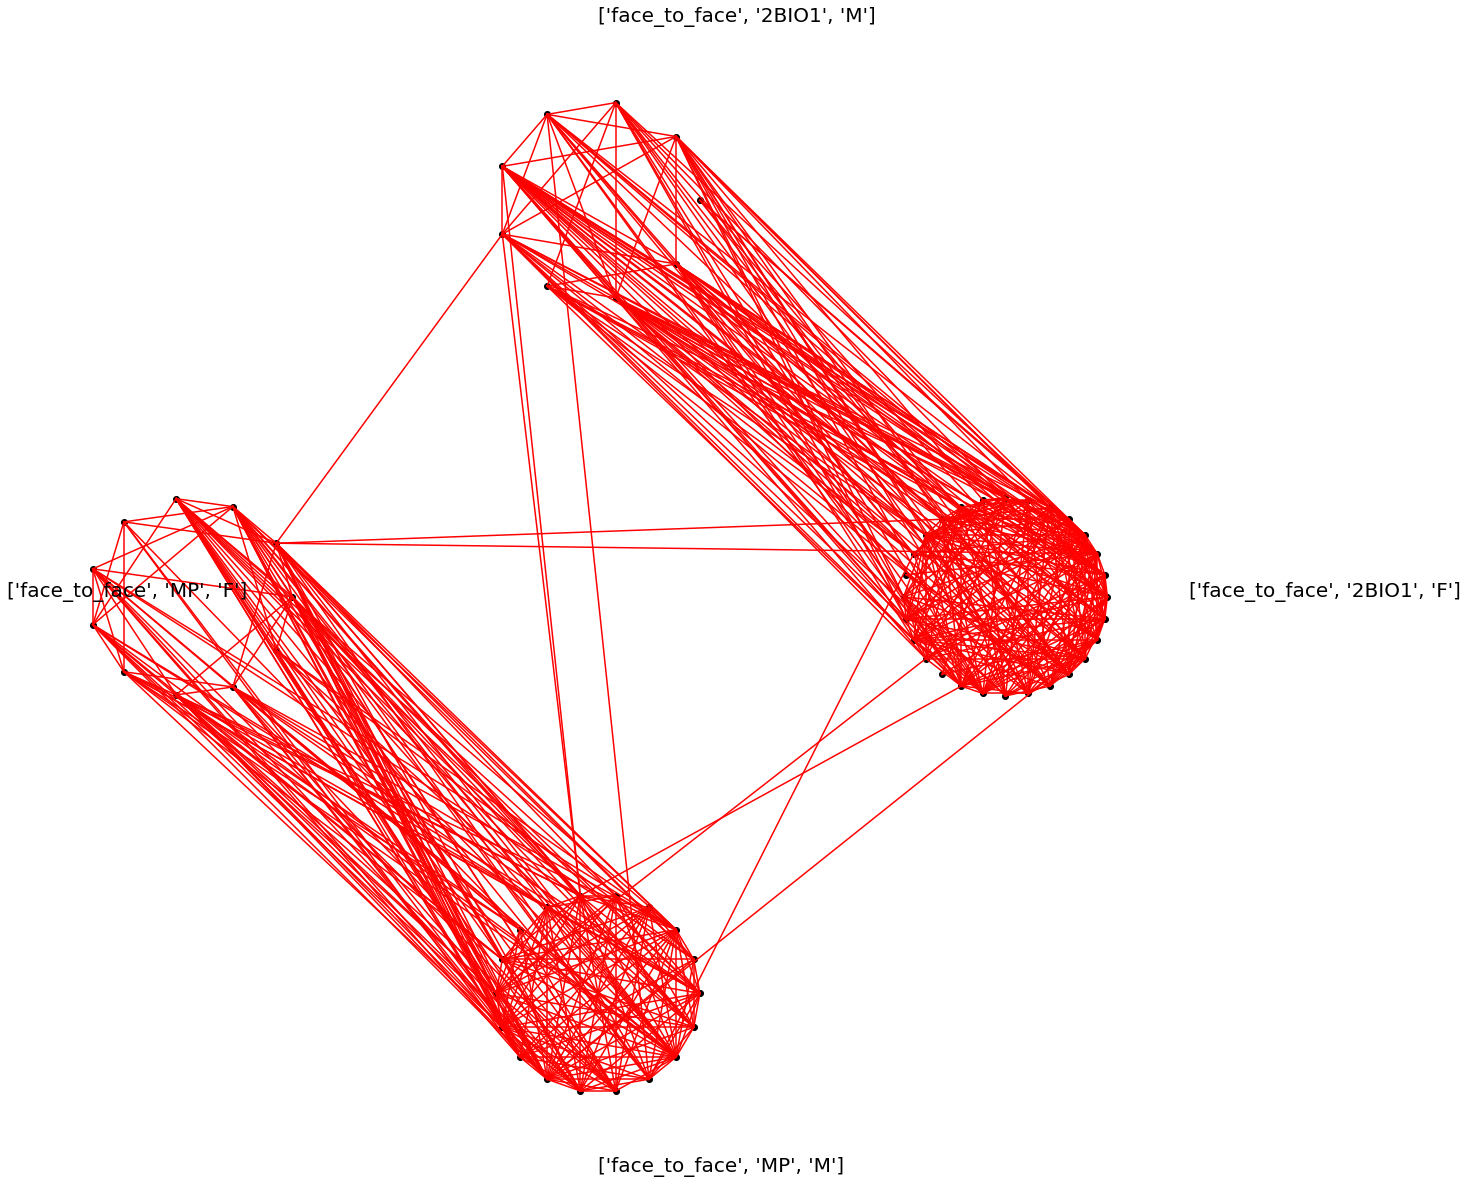
\includegraphics[width=\textwidth]{sousmulticlasseftf.png}
		\captionsetup{margin=10pt}
		\caption{\textbf{Visualisation du sous graphe multicouches induit des relations \texttt{`face to face'}, entre les élèves de deux classes} : les \texttt{`2BIO1'} et les \texttt{`MP'}.}
	\end{minipage}
	\caption{\textbf{Comparaison entre différents aspects du graphe multicouches. } On peut s'intéresser à la pertinence de séparer filles et garçons en différentes couches. En revanche, la séparation entre différentes classes semble être justifiée.}
	\label{induit}
\end{figure}
	
	
\subsubsection{Étude des densités intra et inter-couches pour plusieurs aspects}
	On peut alors se demander en regardant ces interactions (\cref{induit,completinduit}) , si le partitionnement différenciant les femmes et les hommes est \og visible \fg{} d'un point de vue des interactions.

Nous avons donc calculé la densité des relations femmes/hommes comparée aux densités des relations au sein des hommes et des femmes, au fil des jours. Cette densité correspond à la probabilité, prenant un temps aléatoire et deux n\oe{}uds aléatoires, ces n\oe{}uds soient reliés par une arête.

Au sein des hommes, des femmes, ou pour la densité totale, on calcule donc:$$
\delta = \frac{\sum_{u,v \in V\otimes V} |T_{uv}|}{\sum_{u,v \in V \otimes V}|T_u\cap T_v|} = \frac{2|E|}{|T|(|V|(|V|-1))}$$
et dans le graphe biparti des interactions hommes-femmes, la densité est:
$$\delta_{biparti}=\frac{\sum_{u,v \in V_f \times V_h} |T_{uv}|}{\sum_{u,v \in V_f \times V_h}|T_u\cap T_v|}=\frac{|E|}{|T||V_f||V_h|}$$
\begin{figure}[H]
	\centering
	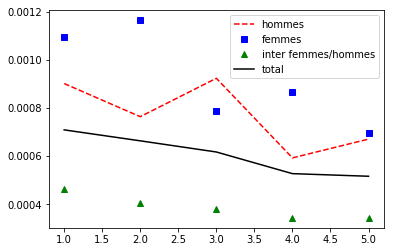
\includegraphics[width=0.5\textwidth]{compfg.png}
	\caption{Densité des relations au sein des femmes, des hommes, des relations inter-hommes/femmes, et des relations en général prise chaque jour de la semaine.}
	\label{densitesemaine}
\end{figure}

Nous voyons qu'une tendance se confirme: les relations sont plus denses au sein d'un même sexe qu'en moyenne, et les relations inter-sexes sont moins denses qu'en moyenne. Nous avons donc tracé les mêmes densités pour des graphes multicouches sous-jacents correspondant aux jours de la semaine (\cref{dsj}). Nous obtenons les mêmes tendances mais moins \og contrastées \fg{} puisqu'une relation de longue durée \og pèse \fg{} autant qu'une relation de courte durée qui a pu être enregistrée \og par hasard \fg{}, mais qui ne reflète pas une réelle interaction. La composante \stg{} dans notre \stgm{} nous permet donc d'obtenir un résultat plus \og fin \fg{} que la projection en graphe aggrégé.

\begin{figure}[H]
	\centering
	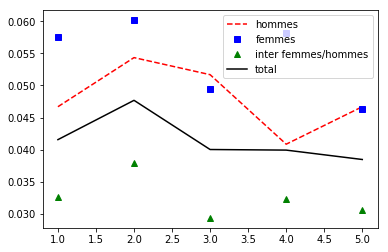
\includegraphics[width=0.5\textwidth]{densitesj.png}
	\caption{Densité des graphes sous-jacents pour les 5 jours de la semaine.}
	\label{dsj}
\end{figure}

Nous avons comparé les différentes densités pour les aspects \texttt{`facebook'} et \texttt{`frienship'}. Nous avons alors relevé les mêmes tendances, et même nettement plus accentuées pour les relations amicales, où les relations intra-hommes passent en dessous de la moyenne (\cref{comp})

\begin{figure}[H]
	\centering
	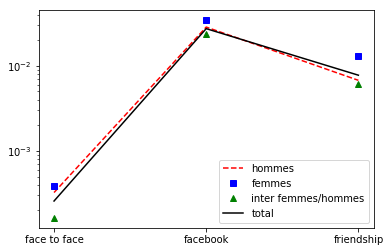
\includegraphics[width=0.5\textwidth]{comparatif.png}
	\caption{Comparatif des densités pour les relations \texttt{`face to face'}, \texttt{`facebook'} et \texttt{`friendship'} en échelle logarithmique, pour les aspects \texttt{`hommes'}, \texttt{`femmes'}, le graphe inter-couche \texttt{`hommes'/`femmes'} et le graphe en entier.}
	\label{comp}
\end{figure}  

Nous avons donc montré que les outils créés pour les \stgms{} peuvent servir pour analyser des interactions entre individus de façon plus nuancée. La densité associée aux sous-\stg{} inter-couches et intra-couches sert à caractériser des interactions de différents types entre plusieurs groupes d'individus.


\section{Conclusions et perspectives}

    Nous avons donc présenté notre nouvel objet ainsi que les raisons qui ont mené à sa création. Nous avons formalisé plusieurs notions pour nous permettre d'extraire des graphes d'intérêt et de prendre des mesures, et nous avons montré un exemple d'utilisation de ces notions grâce à un jeu de données.
    
    Pour la suite du stage, nous avons trouvé deux jeux de données très différents pouvant se prêter à notre étude, et permettant des applications diverses.
    Le premier recense les personnages, dialogues et lieux des films StarWars, ainsi que leurs interactions dans le temps. Le but sera de \og trouver \fg{} quels sont les personnages, sujets et lieux \og principaux \fg{} ou \og centraux \fg{}, en adaptant des méthodes d'intrication~\cite{intrication}, existantes pour les graphes multicouches, aux \stgms{}.
    Le second recense tous les vols sur le sol américain entre 1987 et aujourd'hui, pour différentes compagnies aériennes (représentant les différentes couches). Cette fois-ci, il nous faudra adapter le modèle de \stgm{} au même objet mais dans lequel les liens sont \og instantanés \fg{} et coûtent un temps $\gamma$ à être parcourus. Le but sera ensuite d'étudier la \og centralité \fg{} des aéroports ou des compagnies aériennes, grâce à des mesures multicouches, des simulations de trajets aléatoires et peut-être une adaptation du PageRanking à notre nouvel objet, en nous inspirant de~\cite{centraliteMulti}.
    
    Bien que la notion de \stgms{} semble naturellement adaptée en théorie à de nombreux jeux de données, peu d'entre eux sont en fait accessibles à l'heure actuelle. En effet, le formalisme n'existant pas, il n'a probablement pas semblé utile de collecter autant d'informations dans les jeux de données que le type des relations et surtout les temps d'interaction. Mais avec le nombre croissant de \og big data \fg{} à notre disposition, il est très probable que nous ayons accès de plus en plus souvent à ce genre de données.

    \nocite{*}
    \bibliographystyle{plain}
	\bibliography{rapport}

\end{document}
